%%%%%%%%%%%%%%%%%%%%%%%%%%%%%%%%%%%%%%%%%%%%%%
% An example of a lab report write-up.
%%%%%%%%%%%%%%%%%%%%%%%%%%%%%%%%%%%%%%%%%%%%%% 
% This is a combination of several labs that I have done in the past for 
% Computer Engineering, so it is not to be taken literally, but instead used as 
% a great starting template for your own lab write up.  When creating this 
% template, I tried to keep in mind all of the functions and functionality of 
% LaTeX that I spent a lot of time researching and using in my lab reports and 
% include them here so that it is fairly easy for students first learning LaTeX
% to jump on in and get immediate results.  However, I do assume that the 
% person using this guide has already created at least a "Hello World" PDF 
% document using LaTeX (which means it's installed and ready to go). 
%
% My preference for developing in LaTeX is to use the LaTeX Plugin for gedit in 
% Linux.  There are others for Mac and Windows as well (particularly MikTeX).  
% Another excellent plugin is the Calc2LaTeX plugin for the OpenOffice suite.  
% It makes it very easy to create a large table very quickly.  
%
% Professors have different tastes for how they want the lab write-ups done, so 
% check with the section layout for your class and create a template file for 
% each class (my recommendation).
%
% Also, there is a list of common commands at the bottom of this document.  Use
% these as a quick reference.  If you'd like more, you can view the "LaTeX Cheat
% Sheet.pdf" included with this template material. 
%
% (c) 2009 Derek R. Hildreth <derek@derekhildreth.com> http://www.derekhildreth.com 
% This work is licensed under the Creative Commons Attribution-NonCommercial-ShareAlike License. To view a copy of this license, visit http://creativecommons.org/licenses/by-nc-sa/1.0/ or send a letter to Creative Commons, 559 Nathan Abbott Way, Stanford, California 94305, USA.
%%%%%%%%%%%%%%%%%%%%%%%%%%%%%%%%%%%%%%%%%%%%%%
\documentclass[aps,letterpaper,10pt]{article}

\setlength{\parindent}{0in}

\usepackage{graphicx} % For images
\usepackage{float}    % For tables and other floats
\usepackage{verbatim} % For comments and other
\usepackage{amsmath}  % For math
\usepackage{amssymb}  % For more math
\usepackage{fullpage} % Set margins and place page numbers at bottom center
\usepackage[italian]{babel} % Set Italian language
\usepackage{listings} % For source code
\usepackage{subfig}   % For subfigures
\usepackage[usenames,dvipsnames]{color} % For colors and names
\usepackage[pdftex]{hyperref}           % For hyperlinks and indexing the PDF
\hypersetup{ % play with the different link colors here
    colorlinks,
    citecolor=blue,
    filecolor=blue,
    linkcolor=blue,
    urlcolor=blue % set to black to prevent printing blue links
}

\definecolor{mygrey}{gray}{.96} % Light Grey
\lstset{ 
	language=[ISO]C++,              % choose the language of the code ("language=Verilog" is popular as well)
   	tabsize=3,						% sets the size of the tabs in spaces (1 Tab is replaced with 3 spaces)
	basicstyle=\tiny,               % the size of the fonts that are used for the code
	numbers=left,                   % where to put the line-numbers
	numberstyle=\tiny,              % the size of the fonts that are used for the line-numbers
	stepnumber=2,                   % the step between two line-numbers. If it's 1 each line will be numbered
	numbersep=5pt,                  % how far the line-numbers are from the code
	backgroundcolor=\color{mygrey}, % choose the background color. You must add \usepackage{color}
	%showspaces=false,              % show spaces adding particular underscores
	%showstringspaces=false,        % underline spaces within strings
	%showtabs=false,                % show tabs within strings adding particular underscores
	frame=single,	                % adds a frame around the code
	tabsize=3,	                    % sets default tabsize to 2 spaces
	captionpos=b,                   % sets the caption-position to bottom
	breaklines=true,                % sets automatic line breaking
	breakatwhitespace=false,        % sets if automatic breaks should only happen at whitespace
	%escapeinside={\%*}{*)},        % if you want to add a comment within your code
	commentstyle=\color{BrickRed}   % sets the comment style
}

% Make units a little nicer looking and faster to type
\newcommand{\Hz}{\textsl{Hz}}
\newcommand{\KHz}{\textsl{KHz}}
\newcommand{\MHz}{\textsl{MHz}}
\newcommand{\GHz}{\textsl{GHz}}
\newcommand{\ns}{\textsl{ns}}
\newcommand{\ms}{\textsl{ms}}
\newcommand{\s}{\textsl{s}}



% TITLE PAGE CONTENT %%%%%%%%%%%%%%%%%%%%%%%%
% Remember to fill this section out for each
% lab write-up.
%%%%%%%%%%%%%%%%%%%%%%%%%%%%%%%%%%%%%%%%%%%%%
\newcommand{\univ}{Univerisit\`a degli Studi di Padova}
\newcommand{\faculty}{Facolt\`a di Scienze MM. FF. NN.}
\newcommand{\labtitle}{Sistemi Concorrenti e Distribuiti}
\newcommand{\titletrack}{Software per Simulare Match Calcistici}
\newcommand{\authorname}{dott. Paolo Carletto}
\newcommand{\professor}{dott. Tullio Vardanega}
\newcommand{\classno}{622276}
\newcommand{\aayear}{2011/12}
\newcommand{\logo}{images/soccerball.png}
\newcommand{\unilogo}{images/unipd-logo.png}
% END TITLE PAGE CONTENT %%%%%%%%%%%%%%%%%%%%


\begin{document}  % START THE DOCUMENT!

% TITLE PAGE %%%%%%%%%%%%%%%%%%%%%%%%%%%%%%%%%%%%%%
% If you'd like to change the content of this,
% do it in the "TITLE PAGE CONTENT" directly above
% this message
%%%%%%%%%%%%%%%%%%%%%%%%%%%%%%%%%%%%%%%%%%%%%%%%%%%
\begin{titlepage}
\begin{center}
{\Large \textsc{\univ} \\ \vspace{4pt}}
{\Large \textsc{\faculty} \\ \vspace{4pt}}
{\Large \textsc{\labtitle} \\ \vspace{4pt}} 
\rule[13pt]{\textwidth}{1pt} \\ \vspace{55pt}

\begin{figure}[h]
	\begin{center}
		\includegraphics[width=0.33\textwidth]{\logo}
	\end{center}
\label{graph}
\end{figure}
\vspace{40pt}

\Large \textbf{\titletrack} \\ \vspace{15pt}

{\large \textbf{Autore:} \authorname \\ \vspace{10pt}
\textbf{Matricola:} \classno \\ \vspace{10pt}
\textbf{Docente:} \professor \\ \vspace{10pt}
\textbf{A.A.} \aayear  \\ \vspace{10pt}
\textbf{03 gennaio 2011}} \\ \vspace{10mm}
\mbox{\includegraphics[width=80px]{\unilogo}}
\end{center}
\end{titlepage}
% END TITLE PAGE %%%%%%%%%%%%%%%%%%%%%%%%%%%%%%%%%%


\tableofcontents
\newpage

\section{Introduzione}

\subsection{Tema}

Il tema del progetto \`e un simulatore software di una partita di calcio. \vspace{3mm}

Il sistema software deve supportare almeno le seguenti caratteristiche:
\begin{itemize}
	\item Gli utenti devono essere in grado di giocare un singolo match; il supporto per la giocabilit\`a di una serie di partite con calendari e regole associate \`e facoltativo e pu\`o essere omesso;
	\item La variante scelta del gioco deve essere configurabile in tutti i parametri rilevanti, consentendo uno dei formati classici del calcetto a 5, 7 e il canonico 11 gicatori;
	\item I componenti delle squadre saranno caratterizzati da caratteristiche configurabili individualmente almeno per capacit\`a tecniche e tattiche, velocit\`a, parametri fisici tra cui anche la stanchezza; alcuni di questi parametri devono essere dinamici ed evolvere con la partita secondo una logica programmata;
	\item Ogni squadra deve avere un manager (software) in grado di configurare la formazione iniziale dei giocatori, la tattica iniziale e di impartire comandi per cambiamenti tattici e sostituzioni, tutti soggetti alle regole del gioco come definito nello standard corrispondente;
	\item Ogni squadra deve giocare secondo la tattica comandata dal manager; variazioni sono ammesse nella misura in cui risultano dalle caratteristiche programmabili dei giocatori;
	\item Ogni partita ha un arbitro (software) indipendente e 2 o 3 assistenti (software) subordinati che controllano il gioco e garantiscono che le norme vengano rispettate; il comportamento e le prestazioni dell'arbitro e degli assistenti non necessitano di mostrare i limiti fisici tipiche degli esseri umani;
\end{itemize}

Il sistema software deve includere almeno:
\begin{itemize}
	\item Un software di base, centralizzato o distribuito, che implementi tutta la logica della simulazione;
	\item Un pannello grafico di sola lettura per la visualizzazione del campo di calcio, i giocatori, la palla, l'arbitro e gli assistenti; per le figure umane in campo \`e sufficiente a rappresentarle come puntini numerati che si muovono sul display senza ricorrere a sofisticati rendering grafici, come in una visione di un tavolo Subbuteo visto dall'alto;
	\item Due distinti pannelli grafici di lettura-scrittura per permettere all'utente di influenzare l'azione altrimenti indipendente del team manager; il pannello deve visualizzare i parametri attuali per ogni giocatore; la frequenza di aggiornamento dei display saranno configurabili dall'utente;
	\item Un pannello grafico di sola lettura per la visualizzazione di statistiche configurabili dall'utente; la frequenza di aggiornamento di questo display sar\`a configurabile dall'utente;
	\item Il nucleo del software deve essere sviluppato in Ada. La progettazione del software deve permettere la sostituzione a piacimento degli algoritmi principali: in altre parole, il sistema software deve essere il pi\`u modulare, configurabile e scalabile possibile. Queste qualit\`a contribuiranno alla valutazione;
	\item I pannelli grafici possono essere programmati in qualsiasi linguaggio che i partecipanti considereranno idonei allo scopo. La bellezza grafica dei pannelli sar\`a tuttavia solo un fattore secondario nella valutazione. Ci\`o che importa invece è\`e che l'interazione e il flusso di dati e di controllo tra il nucleo e il software
\end{itemize}
 
\subsection{Requisiti} 

Possiamo riassumere brevemente i requisiti principali del sistema, ricapitolandoli in una tabella riassuntiva esplicativa. Non vengono proposti, nel presente elaborato, nessun tipo di diagramma Use-Case UML in quanto lo scopo del documento non \`e quello di effettuare un'analisi approfondita dei requisiti, ma di individuare le necessit\`a principali che il software deve soddisfare. Si tratta principalmente di riepilogare quanto proposto nel capitolo precedente al fine di schematizzare gli obiettivi principali.

\begin{table}[H]
\begin{center}
	\begin{tabular}{|l|l|l|}
		\hline
		\textbf{Requisito} & \textbf{Descrizione} & \textbf{Obbligatorio} \\ \hline \hline
		R01 & Possibilit\`a da parte dell'utente di giocare un singolo match & S\`i \\ \hline
		R02 & Configurabilit\`a dei parametri principali & S\`i \\ \hline
		R03 & Configurabilit\`a dei parametri fisici dei giocatori & S\`i \\ \hline
		R04 & Dinamicit\`a delle caratteristiche ed evoluzione durante il match & S\`i \\ 
		& (Es: stanchezza) & \\ \hline
		R05 & Presenza per ogni squadra di un manager & S\`i \\ \hline
		R06 & Il manager gestisce le configurazioni della squadra in campo  & S\`i \\ \hline
		R07 & I giocatori giocano sulla base delle decisioni del manager & S\`i \\ \hline
		R08 & Presenza di un arbitro che controlla il rispetto delle regole & S\`i \\ \hline
		R09 & Utilizzo di un processo per ogni singolo giocatore in campo & S\`i \\ \hline
 		R10 & Distribuzione del sistema su diversi calcolatori & S\`i \\ \hline
		\end{tabular}
\end{center}
\caption{La lista dei requisiti obbligatori del sistema.}
\end{table}

La colonna obbligatorio indica la necessit\`a o meno del requisito al fine del funzionamento del sistema. Tutti i requisiti opzionali devono essere intesi come caratteristiche non necessarie all'implementazione di base del sistema, ma forniscono migliorie non trascurabili al sistema. 

\newpage

\section{Analisi}

\subsection{La Struttura di Gioco}

Il progetto prevede una serie di classi che compongono la struttura del gioco. Il riepilogo presenta gli elementi con una breve descrizione. Ogni singolo elemento verr\`a esaminato nelle sezioni successive entrando nel dettaglio delle varie componenti e dei vari metodi necessari per il corretto funzionamento del sistema.

\begin{table}[H]
\begin{center}
	\begin{tabular}{|l|l|}
		\hline
		\textbf{Elemento} & \textbf{Descrizione} \\ \hline \hline
		%Timer & Regola la durata del match e ne determina la fine. \\ \hline
		Timer & Gestione del tempo di gioco. \\ \hline
		Campo & Dimensioni della superficie di gioco e gestione dei posizionamenti. \\ \hline
		Arbitro & Controlla la regolarit\`a del gioco. \\ \hline
		Manager & Effettua le scelte per la squadra in base agli eventi. \\ \hline
		Giocatore & Gioca la partita nella squadra. \\ \hline
		Pallone & Oggetto condiviso dai giocatori \\ \hline
		\end{tabular}
\end{center}
\caption{La lista degli elementi che compongono il sistema.}
\end{table}

\subsubsection{Timer}

Rappresenta la classe ``Tempo'' del nostro gioco. Si occupa di ricevere l'impostazione iniziale relativa alla durata della partita e di riproporzionare i 90 minuti regolari di un match rispetto ai minuti reali di gioco. Questo permette la gestione univoca del tempo di gioco, dall'inizio alla fine della partita attraverso il risveglio dei processi attivi e lo stop degli stessi al termine della partita.

\subsubsection{Campo}

Le dimesioni del campo dipendono dal numero dei giocatori. Indichiamo le dimensioni ufficiali LNP\footnote{Lega Nazionale Professionisti} sulla base del numero di componenti per ogni singola squadra:

\begin{table}[H]
\begin{center}
	\begin{tabular}{|c|c|c|}
		\hline
		\textbf{Num. Giocatori} & \textbf{Lunghezza} & \textbf{Larghezza} \\ \hline \hline
		5 & 42 & 22 \\ \hline
		7 & 55 & 32 \\ \hline
		8 & 65 & 38 \\ \hline
		11 & 105 & 68\\ \hline
	\end{tabular}
\end{center}
\caption{Le misure standard dei campi da calcio e calcetto.}
\end{table}

Tutte le misure sopra indicate sono da considerarsi espresse in metri\footnote{Un metro è definito come la distanza percorsa dalla luce nel vuoto in un intervallo di tempo pari a 1/299.792.458 di secondo.}. \vspace{3mm}

Le dimensioni del campo da gioco sono fondamentali rispetto al numero dei giocatori in quanto determinano la dimensione del movimento ovvero quanto il giocatore possa procedere in una direzione prima di finire fuori dal bordo.

\begin{figure}[H]
	\begin{center}
		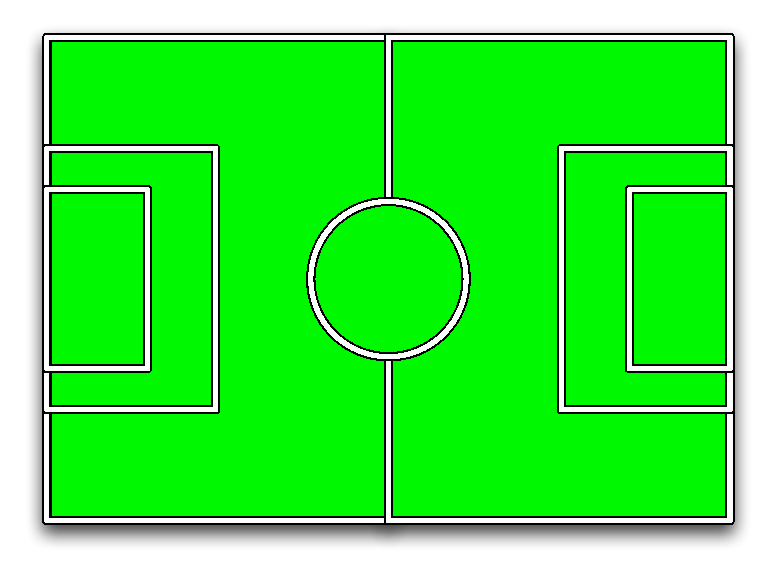
\includegraphics[width=300px]{images/field.pdf}
	\end{center}
\caption{Il campo da gioco}
\end{figure}

Il campo \`e rappresentato attraverso un rettangolo in cui vengono definite le dimensioni dell'area complessiva di gioco e le aree in cui, esclusivamente per i portieri, \`e consentita presa con le mani. La rappresentazione del campo per l'elaboratore \`e una griglia composta da $ 2M \times 2N $ righe di separazione, dove M \`e la lunghezza del campo misurata in metri, mentre N \`e la larghezza. Potenzialmente, suddividendo il reticolato in maglie pi\`u strette, \`e possibile nascondere all'occhio umano il reticolato simulando un movimento fluido piuttosto che scattoso.

\begin{figure}[H]
	\begin{center}
		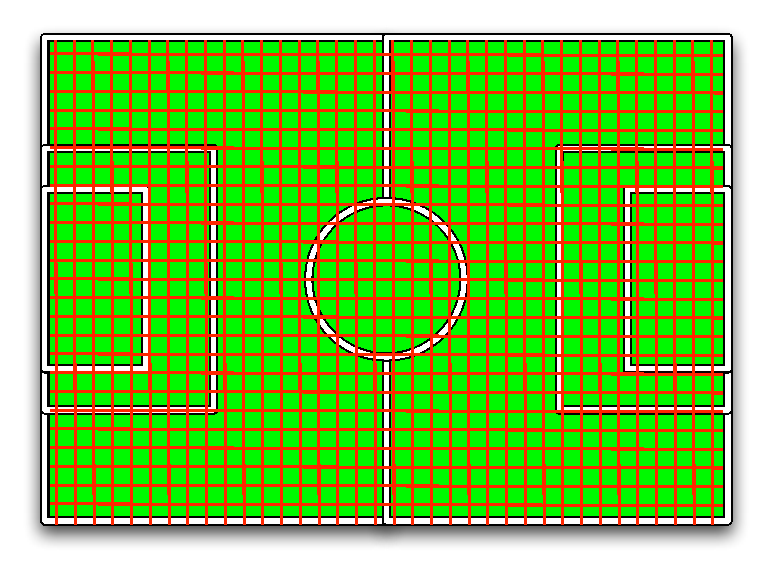
\includegraphics[width=300px]{images/field-web.pdf}
	\end{center}
\caption{Il campo da gioco con il reticolato su cui avvengono i movimenti}
\end{figure}

\subsubsection{Arbitro}

Definiamo l'arbitro come un'entit\`a che assolve il compito di giudicare alcuni eventi che sono segnalati come critici. Variabili aleatorie permettono di simulare il margine di errore decisionale rispetto a tali eventi. \vspace{3mm}

L'arbitro viene assistito da due collaboratori, i guardalinee, che influenzano la decisione attraverso altre 2 variabili aleatorie, spostando il peso della decisione dell'arbitro a favore o contro il fischio. \vspace{3mm}

Non vi sono elementi nel campo da gioco che rappresentano l'arbitro e i suoi collaboratori. Potenzialmente \`e possibile implementare solamente il fischio nel momento in cui viene segnalata una irregolarit\`a di gioco.

\subsubsection{Manager}
\label{man}

Anche il manager della squadra, come per gli arbitri, non \`e rappresentato nel campo da gioco. Non interviene attivamente al gioco sul campo, ma si occupa di seguire la logica con la quale la squadra gioca la partita. Interviene nella scelta della strategia di gioco, nella disposizione iniziale della formazione, nelle eventuali variazioni necessarie a seguito dei risultati in campo e nelle sostituzioni dei vari giocatori all'interno del campo di gioco o tra giocatori in panchina. \vspace{3mm}

Possiamo immaginare facilmente il manager come la mente della squadra che si occupa di interpretare la partita e di mettere la squadra in condizione di vincere.

\subsubsection{Giocatore}

Il giocatore rappresenta la forza in campo che gioca attivamente la partita, cerca di segnare il maggior numero di reti e di subirne il minimo al fine di vincere il match. \vspace{3mm}

Ogni squadra dispone di \emph{n} giocatori in campo di cui necessariamente:

\begin{itemize}
	\item 1 portiere;
	\item 2 difensori;
	\item 2 centrocampisti;
	\item 1 attaccante;
\end{itemize}

Questa disposizione minima obbligatoria evita degli sbilanci eccessivi in favore di un reparto piuttosto che un altro, rendendo i match relativamente equilibrati e giocabili. In caso di calcetto a 5, la disposizione minima \`e leggermente differente per effetto del minor numero di giocatori in campo. \vspace{3mm}

Ogni giocatore \`e contraddistinto da un pallino colorato. La squadra A \`e contraddistinta dal colore blu, mentre la squadra B dal colore rosso.

\begin{figure}[H]
  \centering
  \subfloat[Giocatore A]{
\includegraphics[width=40px]{images/player1.pdf}}  \hspace{1cm}             
  \subfloat[Giocatore B]{
\includegraphics[width=40px]{images/player2.pdf}}
  \caption{I giocatori delle 2 squadre.}
\end{figure}

Il colore della squadra viene assegnato automaticamente in modo casuale durante il processo di inizializzazione della partita.

\subsubsection{Palla}

La palla \`e uno degli elemeni fondamentali del gioco. \`E l'oggetto condiviso dai giocatori e pu\`o essere controllato in ogni istante di tempo da al massimo un giocatore. \vspace{3mm}

Viene mostrato nel campo da gioco come un pallino di colore nero, per contraddistinguerlo dai giocatori.

\begin{figure}[H]
	\begin{center}
		
\includegraphics[width=40px]{images/ball.pdf}
	\end{center}
\caption{Il pallone da gioco}
\end{figure}

Nel momento in cui un giocatore entra in possesso del pallone, per distinguerlo dai compagni, il margine esterno viene rappresentato in grassetto. Questo permette di comprendere a colpo d'occhio quale giocatore detenga il pallone e come si muova con esso.

\begin{figure}[H]
  \centering
  \subfloat[Giocatore A con palla]{
\includegraphics[width=40px]{images/ball-player1.pdf}}  \hspace{1cm}             
  \subfloat[Giocatore B con palla]{
\includegraphics[width=40px]{images/ball-player2.pdf}}
  \caption{I giocatori delle 2 squadre in possesso del pallone.}
\end{figure}

\subsection{I Dettagli di Gioco}

\subsubsection{Movimento}
\label{movimento}

Ogni giocatore \`e in grado di muoversi all'interno del campo da gioco per interagire con gli altri giocatori della squadra, per contrastare gli avversari ed impossessarsi del pallone, per avanzare verso la porta con i compagni o per tirare il pallone nel momento in cui la distanza dalla rete \`e sufficiente per poter compiere un buon tiro e segnare un gol. \vspace{3mm}

\`E stato deciso di semplificare il movimento nei 4 assi fondamentali:

\begin{itemize}
	\item su;
	\item gi\`u;
	\item destra;
	\item sinistra;
\end{itemize}

In questa maniera il giocatore \`e in grado di muoversi negli incroci del reticolato e dichiarare a compagni ed avversari la propria posizione al fine del corretto svolgimento del match. Inoltre, attraverso una serie di piccoli movimenti di questo tipo ogni giocatore \`e in grado di percorrere potenzialmente tutto il campo di gioco.

\begin{figure}[H]
	\begin{center}
		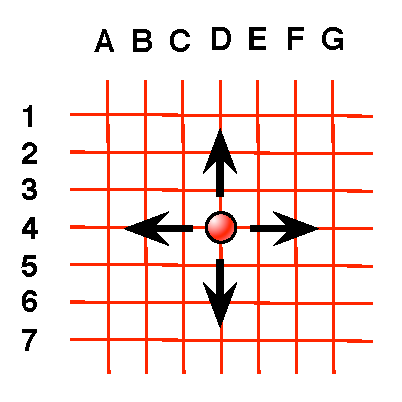
\includegraphics[width=160px]{images/movement.pdf}
	\end{center}
\caption{Gli assi del movimento dei giocatori.}
\end{figure}

\subsubsection{Zone di Movimento}
\label{zone}

Per evitare che i giocatori sbilancino la squadra in modo esagerato \`e stato deciso di creare, per ogni area di gioco, delle ``zone di movimento'' che permettono di mantenere i difensori all'interno della zona di difesa, i centrocampisti entro dei margini di gioco centrali e gli attaccanti al limite del centrocampo. \vspace{3mm}

In questo modo, in caso di contropiede avversario, non rimangono zone troppo scoperte e che gli avversari possono sfruttare a loro favore per effettuare azioni indesiderate.

La difesa muove sempre dalla porta fino al limite del centrocampo, evitando di entrare nella zona di campo avversaria.

\begin{figure}[H]
	\begin{center}
		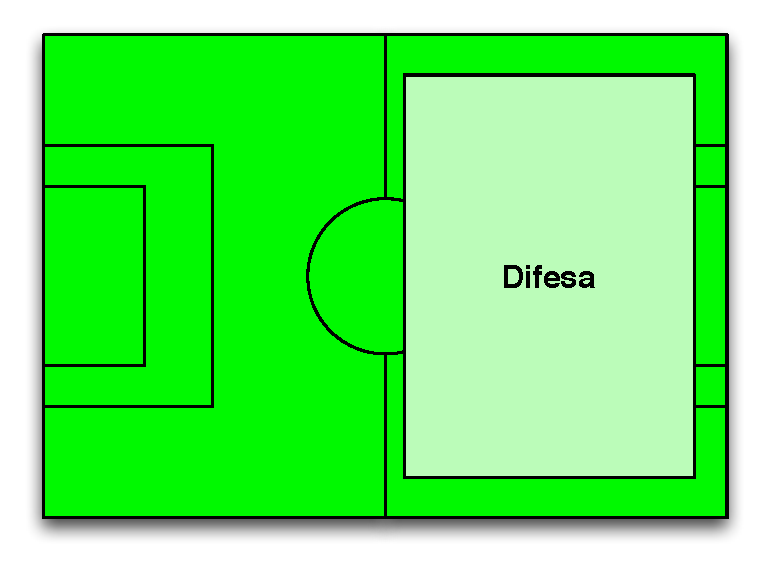
\includegraphics[width=300px]{images/defense.pdf}
	\end{center}
\caption{La zona di movimento dei difensori.}
\end{figure}

Il centrocampo pu\`o muoversi in tutta la parte centrale del campo e nelle fascie laterali per assistere gli attaccanti e i difensori.

\begin{figure}[H]
	\begin{center}
		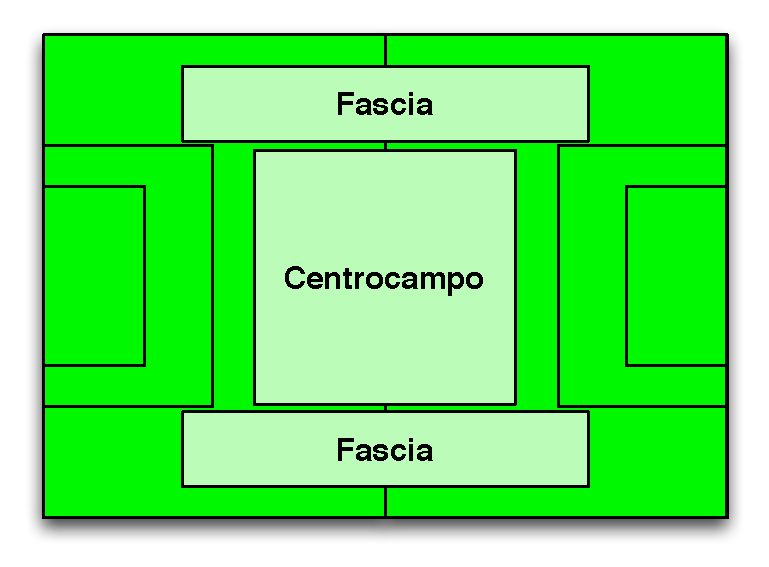
\includegraphics[width=300px]{images/middle.pdf}
	\end{center}
\caption{La zona di movimento dei centrocampisti.}
\end{figure}

Gli attaccanti invece muovono in tutta la zona del campo avversario senza mai retrocedere oltre il limite del centrocampo, per poter intervenire in caso di passaggi da parte dei compagni in caso di contropiede.

\begin{figure}[H]
	\begin{center}
		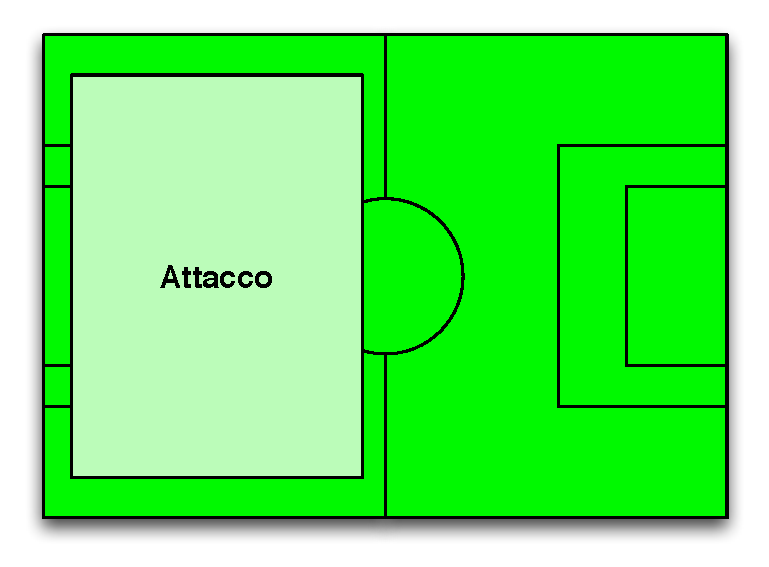
\includegraphics[width=300px]{images/attack.pdf}
	\end{center}
\caption{La zona di movimento degli attaccanti.}
\end{figure}

\subsubsection{I Giocatori}

Ogni giocatore, oltre al movimento all'interno del campo \`e in grado di effettuare alcune azioni di base ed in particolar modo legate ad alcune condizioni fondamentali:

\begin{itemize}
	\item possesso del pallone da parte della propria squadra:
		\begin{itemize}
			\item del giocatore stesso
			\item di un compagno
		\end{itemize}
	\item possesso del pallone da parte degli avversari
\end{itemize}
	
Definiamo con il termine \textit{logica} una modalit\`a di gioco relativa ad ogni singolo giocatore e legata alle condizioni di cui sopra. \vspace{3mm}

Elenchiamo brevemente le possibilit\`a che un giocatore pu\`o trovarsi a dover affrontare, analizzandole poi dettagliatamente nei paragrafi successivi:

\begin{enumerate}
	\item il giocatore ha la palla:
		\begin{itemize}
			\item logica di passaggio
			\item logica di tiro
			\item logica di avanzamento
			\item logica di posizione
		\end{itemize}
	\item la squadra ha la palla:
		\begin{itemize}
			\item logica di smarcatura
			\item logica di avanzamento
			\item logica di posizione
		\end{itemize}
	\item gli avversari hanno la palla:
		\begin{itemize}
			\item logica di indietreggiamento
			\item logica di contrasto
			\item logica di posizione
		\end{itemize}
	\item il giocatore in porta:
		\begin{itemize}
			\item logica di contrasto (sull'attaccante)
			\item logica di parata (solo su tiro avversario)
			\item logica di posizione
		\end{itemize}
\end{enumerate}

\newpage

\section{Applicazioni delle Logiche}

Nella presente sezione analiziamo le formule ed i coefficenti che permettono di determinare, rispetto all'elenco visto precedentemente, le varie azioni che i giocatori possono compiere ed i risultati a cui possono portare. Come abbiamo detto, utilizzeremo il termine ``logica'' per definire una modalit\`a con cui il giocatore determina le possibilit\`a di gioco, sceglie l'azione migliore e la effettua. \vspace{3mm}

Cominciamo definendo un particolare fondamentale: la ``visibilit\`a'' del giocatore. \vspace{3mm}

Con visibilit\`a intendiamo la cognizione dello stato di gioco nell'istante \emph{t} da parte del giocatore in questione. Per semplicit\`a \`e stato deciso di definire con ``visibilit\`a'' un quadrato di lato \emph{x} (con x dispari) e il giocatore oggetto della funzione risiede nell'intersezione centrale. Questo permette al giocatore di conoscere la situazione di compagni ed avversari per tutte le celle contenute nel quadrato. \vspace{3mm}

\begin{figure}[H]
	\begin{center}
		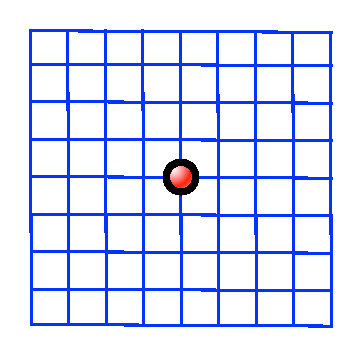
\includegraphics[width=160px]{images/vision.pdf}
	\end{center}
\caption{La ``visibilit\`a'' dei giocatori in gioco.}
\end{figure}

Inoltre \`e possibile rendere il parametro \emph{x} soggettivo rispetto ad ogni giocatore, il che permette a giocatori come il regista di avere una grande visione di gioco rispetto a difensori ed attaccanti. \vspace{3mm}

Tutti i movimenti e i posizionamenti dei giocatori che verranno affrontati nei prossimi capitoli sono sempre da intendersi legati ai ruoli che i giocatori assumono nel campo e alle aree di movimento a cui sono vincolati. Si faccia riferimento alla sezione \ref{zone} per i dettagli delle zone in cui i giocatori sono liberi di muovere. \vspace{3mm}

In tutto il capitolo trascureremo ogni aspetto legato alla concorrenza, tematica che verr\`a affrontata nel dettaglio al capitolo \ref{concorrenza}.

\subsection{Giocatore con Palla}

Il caso pi\`u complesso che possiamo affrontare \`e quello legato al possesso di palla da parte del giocatore. In questa casistica dobbiamo risolvere la maggior parte dei problemi legati alle scelte dei giocatori e determinare le regole con cui avanzano, tirano o passano il pallone ai compagni di squadra. \vspace{3mm}

La priorit\`a con cui un giocatore effettua un'azione \`e:

\begin{enumerate}
	\item tiro in porta
	\item passaggio ad un compagno
	\item avanzamento con palla
	\item mantenimento della posizione
\end{enumerate}

Questo perch\`e se il giocatore vede la porta, effettua un tiro per tentare di segnare una rete. Altrimenti, il passaggio \`e il metodo pi\`u rapido per muovere velocemente la palla ed avanzare verso la porta. In caso non ci sia visione della porte e non ci siano compagni liberi a portata, si processa un avanzamento di posizione. Il mantenimento della posizione \`e una casistica limite che cercheremo sempre di evitare, ma che ci permetter\`a di risolvere situazioni complicate.

\subsubsection{Logica di Tiro}
\label{tiro}

La prima logiche che andiamo ad analizzare \`e quella legata al tiro in porta. \vspace{3mm}

Un giocatore che inizia la logica di tiro ha sicuramente visibilit\`a sulla porta e pertanto non ne \`e relativamente distante.

\begin{figure}[H]
	\begin{center}
		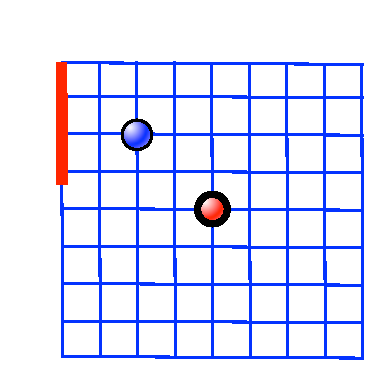
\includegraphics[width=160px]{images/vision1.pdf}
	\end{center}
\caption{Giocatore con palla e visione della porta (linea rossa).}
\end{figure}

Il tiro pu\`o essere un buon tiro o un tiro mediocre. Inoltre pu\`o essere troppo potente o troppo debole e pu\`o venir parato dal portiere avversario. Per simulare un comportamento realistico del tiro, andiamo a considerare alcuni fattori fondamentali:

\begin{itemize}
	\item potenza
	\item precisione
	\item distanza
\end{itemize}

Questi 3 coefficienti fortemente soggettivi rispetto al giocatore e alla posizione, vengono combinati assieme in un'equazione per produrre un coefficiente che verr\`a valutato assieme al coefficiente di parata del portiere (che vedremo in seguito nella sezione \ref{parata}) per determinare il successo o il fallimento del tiro e la conseguente rete della squadra. \vspace{3mm}

L'equazione \`e composta da $$ T_1 = \frac{potenza}{100} \cdot \frac{precisione}{100} \cdot \left( 1-\frac{distanza}{diagonale} \right) $$ dove potenza \`e il valore di potenza del giocatore espresso con un valore da 1 a 100, precisione \`e la precisione di tiro, anch'essa espressa con un valore da 1 a 100, mentre l'ultimo coeffienciente \`e il risultato del rapporto inverso tra la distanza del giocatore dalla porta e la diagonale del campo. \vspace{3mm}

Per dare un'idea di come varino i vari coefficienti ne esprimeremo alcuni campioni nella tabella sottostante ed andremo a definire che cosa rappresentano in termini di gioco.

\begin{table}[H]
\begin{center}
	\begin{tabular}{|c|c|c||c|}
		\hline
		\textbf{Potenza} & \textbf{Precisione} & \textbf{Distanza} & \textbf{Coefficiente} \\ \hline \hline
			0.3 & 0.3 &	0.3 & 0.027 \\ \hline
			0.3 & 0.3 & 0.6 & 0.054 \\ \hline
			0.3 & 0.3 & 0.9 & 0.081 \\ \hline
			0.3 & 0.6 & 0.3 & 0.054 \\ \hline
			0.3 & 0.6 & 0.6 & 0.108 \\ \hline
			0.3 & 0.6 & 0.9 & 0.162 \\ \hline
			0.3 & 0.9 & 0.3 & 0.081 \\ \hline
			0.3 & 0.9 & 0.6 & 0.162 \\ \hline
			0.3 & 0.9 & 0.9 & 0.243 \\ \hline
			0.6 & 0.3 & 0.3 & 0.054 \\ \hline
			0.6 & 0.3 & 0.6 & 0.108 \\ \hline
			0.6 & 0.3 & 0.9 & 0.162 \\ \hline
			0.6 & 0.6 & 0.3 & 0.108 \\ \hline
			0.6 & 0.6 & 0.6 & 0.216 \\ \hline
			0.6 & 0.6 & 0.9 & 0.324 \\ \hline
			0.6 & 0.9 & 0.3 & 0.162 \\ \hline
			0.6 & 0.9 & 0.6 & 0.324 \\ \hline
			0.6 & 0.9 & 0.9 & 0.486 \\ \hline
			0.9 & 0.3 & 0.3 & 0.081 \\ \hline
			0.9 & 0.3 & 0.6 & 0.162 \\ \hline
			0.9 & 0.3 & 0.9 & 0.243 \\ \hline
			0.9 & 0.6 & 0.3 & 0.162 \\ \hline
			0.9 & 0.6 & 0.6 & 0.324 \\ \hline
			0.9 & 0.6 & 0.9 & 0.486 \\ \hline
			0.9 & 0.9 & 0.3 & 0.243 \\ \hline
			0.9 & 0.9 & 0.6 & 0.486 \\ \hline
			0.9 & 0.9 & 0.9 & 0.729 \\ \hline
		\end{tabular}
\end{center}
\caption{Alcuni valori campione per il coefficiente di tiro (media 0.216).}
\end{table}

E' facile comprendere osservando la tabella che al crescere delle carratteristiche ci siano differenti effetti sul tiro: un tiro pu\`o essere molto potente (ultimi risultati in basso) ma non efficace perch\`e poco preciso ed effettuato da distanze troppo elevate. Inoltre pu\`o essere molto preciso e puntare all'incrocio dei pali, ma non sufficientemente potente o magari effettuato da troppo distante e facilmente parabile dal portiere. \vspace{3mm}

Chiameremo il valore ottenuto come $T_1$ e dovr\`a essere confrontato con il risultato del calcolo relativo alla parata per determinare il successo del tiro. \vspace{3mm}

Il fattore aleatorio \`e stato escluso dal calcolo in quanto potrebbe complicare ulteriormente i conteggi e rendere difficile segnare una rete. Non sarebbe per\`o complesso introdurre il classico fattore \emph{c} generando un numero casuale e incrementando o moltiplicando il coefficiente ottenuto precendentemente per \emph{c} ottenendo un coefficiente $T_2$ maggiormente influenzato da leggi pseudo-casuali.

\subsubsection{Logica di Passaggio}

Un giocatore che ha la palla pu\`o decidere di passare il pallone ad un compagno libero. La logica con cui avviene il passaggio \`e legato all'avanzamento verso la porta avversaria. Non \`e per\`o sempre possibile avanzare rispetto alla porta per effetto delle distanze dei giocatori avversari all'uomo a cui si vorrebbe passare il pallone. \vspace{3mm}

Anche in questo caso entra in gioco la ``visibilit\`a'' del giocatore e la sua capacit\`a di vedere compagni liberi nelle vicinanze. 

\begin{figure}[H]
	\begin{center}
		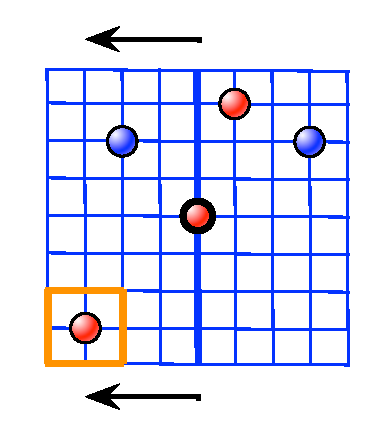
\includegraphics[width=160px]{images/vision2.pdf}
	\end{center}
\caption{Giocatore con palla e visione di compagni ed avversari.}
\end{figure}

Il giocatore in possesso di palla, valuta la posizione del giocatore pi\`u vicino e pi\`u avanzato rispetto a se, controlla che sia libero entro un certo raggio ed eventualmente passa il pallone. L'equazione che regola il passaggio, in questo caso \`e pi\`u semplice della precedente e garantisce quasi sempre il buon fine del passaggio al giocatore destiantario entro un intervallo di tempo \emph{t}. In particolare l'equazione \`e influenzata dalla distanza tra chi passa la palla e chi la deve ricevere e dalla precisione del passaggio: $$ P_1 = \left( 1 - \frac{distanza}{diagonale} \right) \cdot \frac{precisione}{100} $$ Nel caso non si raggiunga la soglia, il pallone viene lanciato casualmente in una delle 4 direzioni per un numero variabile di intersezioni. Questo permette potenzialmente alla squadra avversaria di impossessarsi della palla in quanto ne prender\`a il possesso il primo giocatore a venirne in contatto indipendentemente dallo schieramento.

\begin{figure}[H]
	\begin{center}
		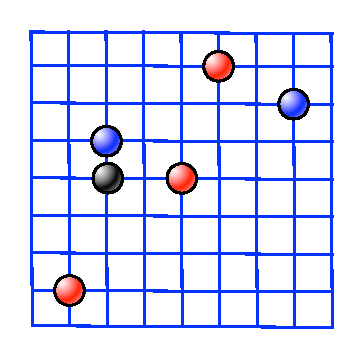
\includegraphics[width=160px]{images/vision3.pdf}
	\end{center}
\caption{Giocatore avversario si avvicina al pallone prima degli altri.}
\end{figure}

Il buon fine del passaggio \`e soggetto al superamento della soglia minima per il passaggio pari a 0.3. Il valore di soglia \`e stato approssimato secondo il criterio per cui un passaggio non avviene mai a distanze elevate e la precisione dei giocatori non dovrebbe essere mai troppo bassa. 

\begin{table}[H]
\begin{center}
	\begin{tabular}{|c|c||c|}
		\hline
		\textbf{Precisione} & \textbf{Distanza} & \textbf{Coefficiente} \\ \hline \hline
			0.3 & 0.6 & 0.18 \\ \hline
			0.3 & 0.8 & 0.24 \\ \hline
			0.6 & 0.6 & 0.36 \\ \hline
			0.6 & 0.8 & 0.48 \\ \hline
			0.9 & 0.6 & 0.54 \\ \hline
			0.9 & 0.8 & 0.72 \\ \hline
	\end{tabular}
\end{center}
\caption{Alcuni valori campione per il coefficiente di passaggio (soglia 0.3).}
\end{table}

Come si pu\`o facilmente vedere dalla tabella, per passaggi molto ravvicinati ($\frac{1}{4}$ della diagonale del campo), anche con una precisione molto bassa (intorno a 40 punti) il passaggio avviene con successo. Chiaramente, giocatori pi\`u precisi non sbaglieranno passaggi facili, ma potrebbero comunque avere qualche difficolt\`a in passaggi lunghi a giocatori distanti. \vspace{3mm}

Anche qui, come nel tiro in porta, pu\`o essere introdotto un fattore aleatorio che pu\`o scombinare gli eventi: il fattore \emph{c} pu\`o entrare in calcoleo nell'equazione che assumerebbe la forma: $$ P_1 = \left( 1 - \frac{distanza}{diagonale} \right) \cdot \frac{precisione}{100} \cdot c $$ dove c \`e un numero casuale tra 0,5 e 1,5. Questo potrebbe portare al fallimento di ottimi passaggi e al successo di passaggi inizialmente fallimentari. \vspace{3mm}

Nella logica di passaggio non \`e stato affrontato il passaggio all'indietro ad un compagno di squadra. Questo per un semplice motivo. Se avessimo considerato anche i passaggi all'indietro, avremmo scatenato un meccanismo infinito di passaggi tra giocatori con una piccolissima percentuale d'errore. Potenzialmente gli interi 90 minuti di gioco potrebbero essere spesi in passaggi tra giocatori senza nemmeno un tiro in porta. Forzando il passaggio in avanti costringiamo i giocatori ad avanzare, passare o tirare in porta. In questo modo evitiamo diverse situazioni che possono causare un stallo del gioco inteso come assenza di azioni a causa di una politica non consistente. \vspace{3mm}

\subsubsection{Logica di Avanzamento}
\label{avanzamento}

Un'altra azione a disposizione di un giocatore con la palla che non pu\`o effettuare un tiro e non pu\`o passare la palla \`e quella di avanzare con il pallone verso la porta. Un giocatore pu\`o anche muovere sulla linea verticale verso l'alto o verso il basso, specialmente verso un compagno di squadra che si sta smarcando per ricevere il passaggio del compagno. \vspace{3mm}

Un giocatore potrebbe per\`o continuare con un movimento ripetitivo dall'altro verso il basso e viceversa per tutta la durata della partita. Per evitare una situazione di questo genere, \`e stato scelto di limitare a \emph{y} il numero di movimenti in orizzontale fino al successivo avanzamento verso la porta avversaria. \vspace{3mm}

Per risolvere il problema \`e sufficiente inserire nella classe \emph{Giocatore} una variabile \emph{y} inizializzata al numero di movimenti verticali massimi. Un contatore decrementa il valore di \emph{y} per ogni movimento consecutivo sull'asse verticale. Quando \emph{y} raggiunge il valore 0, l'avanzamento \`e obbligatorio e \emph{y} viene reimpostata al valore iniziale.

\begin{figure}[H]
	\begin{center}
		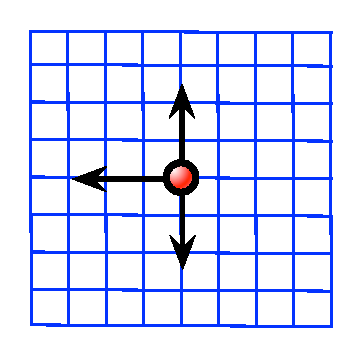
\includegraphics[width=160px]{images/vision4.pdf}
	\end{center}
\caption{Giocatore in fase di movimento con palla.}
\end{figure}

\subsubsection{Logica di Posizione}
\label{posizione}

Il giocatore ha come azione di default in caso di emergenza un'ultima logica che viene utilizzata nel momento in cui nessuna delle logiche precedenti porti ad un risultato: il mantenimento della propria posizione in campo senza alcun tipo di movimento. \vspace{3mm}

\`E una logica che non determina alcuna variazione del gioco, ma che permette di compiere in ogni caso un'azione e di restituire un parametro di ``azione compiuta'' alla classe ``Timer'' per poter procedere nell'invio del successivo istante temporale \emph{t+1}.

\subsection{Squadra con Palla}

Un tipo di logica differente si applica quando il giocatore non \`e direttamente in possesso della palla, ma lo \`e un compagno di squadra. La strategia di movimento del giocatore deve essere finalizzata ad assistere il giocatore con la palla al fine di poter ricevere un passaggio e procedere verso la porta.

\subsubsection{Logica di Smarcatura}

Un giocatore senza palla deve garantire ai compagni di essere libero nel momento in cui sia necessario passare il pallone. \`E fondamentale infatti che assista la squadra nell'avanzamento verso la porta e si proponga per ricevere il pallone ed effettuare a sua volta un'azione. \vspace{3mm}

In questo modo l'azione prioritaria \`e il movimento verso una intersezione distante almeno \emph{n} intersezioni da uno o pi\`u avversari, dando prevalenza ad azioni di avanzamento rispetto a quelle di arretramento in modo da favorire l'attacco verso la porta avversaria.

L'azione di spostarsi verso un punto distante almeno \emph{n} intersezioni consecutive da tutti gli avversari \`e detta ``smarcatura''.

\begin{figure}[H]
	\begin{center}
		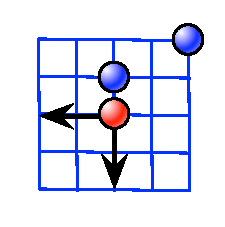
\includegraphics[width=100px]{images/unmark.pdf}
	\end{center}
\caption{Giocatore in fase di smarcatura senza palla.}
\end{figure}

\subsubsection{Logica di Avanzamento}

Nel momento in cui il giocatore risulti gi\`a smarcato rispetto agli avversari si applica la stessa logica di avanzamento che si applica ad un giocatore in possesso di palla: il movimento deve essere direzionato in avanti verso la porta avversaria. Valgono le stesse regole viste nella sezione \ref{avanzamento}.

\subsubsection{Logica di Posizione}

Come gia visto nella sezione \ref{posizione}, anche per il giocatore senza palla esiste un'azione di ``emergenza'' che permette di evitare situazioni di stallo determinate da impossibilit\`a di compiere un movimento nel campo.

\subsection{Avversari con Palla}

Finora abbiamo visto tutte le logiche al possesso del pallone da parte della squadra o del giocatore, ma grossomodo per il 50\% della durata della partita la palla sar\`a in mano ai giocatori avversari e la squadra dovr\`a assumere un atteggiamento difensivo al fine di evitare che gli avversari possano segnare una rete. Analiziamo le logiche di gioco che permettono di difendere la porta.

\subsubsection{Logica di Contrasto}
\label{scontro}

Nel momento in cui gli avversari prendono possesso del pallone, \`e necessario un meccanismo che permetta al giocatore di recuperare il pallone al fine di invertire le parti e portare la propria squadra in fase di attacco. Questa regola \`e definita come logica di contrasto ed \`e rappresentata nel campo di gioco da un contatto fisico tra giocatori. Nel contrasto, i due giocatori si scontrano per potenza e il pi\`u forte prende il controllo del pallone. \vspace{3mm}

\begin{figure}[H]
	\begin{center}
		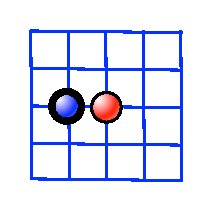
\includegraphics[width=100px]{images/contrast.pdf}
	\end{center}
\caption{Giocatore in fase di contrasto contro un avversario con palla.}
\end{figure}

Il contatto fisico avviene tra due giocatori in posizione ravvicinata, a distanza di un'intersezione l'uno dall'altro. La logica con cui avviene il contrasto viene applicata ad entrambi i giocatori e rispetta la formula: $$ C_1 = \frac{potenza}{100} + c $$ dove potenza \`e la potenza del giocatore e \emph{c} un fattore casuale con valore compreso tra -0.2 e 0.3 che rappresenta un rimpallo a favore o contro il giocatore. \vspace{3mm}

Nel momento in cui avviene il contrasto l'oggetto condiviso viene liberato per l'istante \emph{t} in cui viene valutato il contrasto e poi preso dal giocatore che ottene il valore superiore rispetto al valore di contrasto. \vspace{3mm}

In caso la formula produca due valori uguali, il giocatore in difesa vince il contrasto e prende il controllo della risorsa e il gioco ricomincia. \vspace{3mm}

I dettagli legati alla liberazione della risorsa e alla ripresa della stessa a seguito del contrasto vengono discussi nel capitolo \ref{contrasto}.

\subsubsection{Logica di Indietreggiamento}

Nel momento in cui un giocatore non ha visibilit\`a sul giocatore con la palla pu\`o effettuare una sola azione: indietreggiare a supporto della fase difensiva.

\begin{figure}[H]
	\begin{center}
		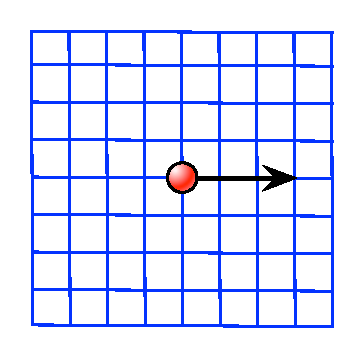
\includegraphics[width=160px]{images/return.pdf}
	\end{center}
\caption{Giocatore in fase di indietreggiamento.}
\end{figure}

In questa maniera, il giocatore si avvicina ai giocatori in difesa, limita le aree di movimento degli avversari in fase di attacco e, in caso di recupero del pallone, si propone per il passaggio da parte dei compagni.

\subsubsection{Logica di Posizione}

Anche nel caso in cui la propria squadra non sia in possesso del pallone, come gia visto nella sezione \ref{posizione}, esiste la solita azione di ``emergenza'' ovvero il mantenimento della propria posizione in campo.

\subsection{Parata del Portiere}

L'unico giocatore eccezionale nel campo di gioco \`e il portiere. Questo particolare giocatore non segue le regole valide per tutti gli altri giocatori nel campo di gioco ma \`e soggetto a delle proprie logiche che lo differenziano nel modo di giocare, di muoversi e di reagire agli eventi come avanzamenti dell'attaccante avversario e al tiro in porta.

\begin{figure}[H]
	\begin{center}
		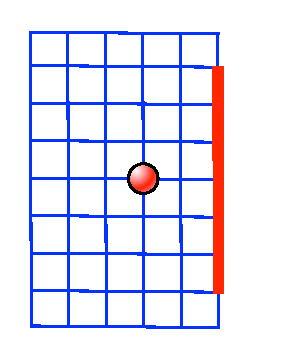
\includegraphics[width=130px]{images/keeper.pdf}
	\end{center}
\caption{Portiere in posizione difensiva.}
\end{figure}

Vediamo nel dettaglio le logiche che ne regolano i movimenti e la posizione.

\subsubsection{Logica di Contrasto}

La logica primaria che permette il movimento del portiere \`e il contrasto con il giocatore avversario. Limitatamente all'area di gioco entro cui il portiere ha la possibilit\`a di muoversi, il portiere cerca il contatto fisico con l'avversario che controlla il pallone. In questo modo pu\`o tentare uno scontro fisico e prendere il controllo del pallone evitando che l'attaccante possa segnare una rete.

\begin{figure}[H]
	\begin{center}
		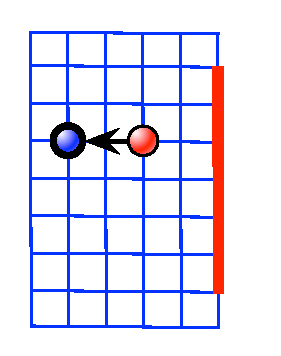
\includegraphics[width=130px]{images/keep-contrast.pdf}
	\end{center}
\caption{Portiere in fase di contrasto.}
\end{figure}

Le regole per la determinazione del contrasto sono uguali a quelle viste nella sezione \ref{scontro}. L'unica differenza \`e relativa al peso del fattore $c$. In questo caso, poich\`e il portiere \`e l'unico giocatore a cui \`e permesso l'intervento con le mani, il valore di $c$ nella formula: $$ C_2 = \frac{potenza}{100} + c $$ varia tra 0 e 0.2, rendendo la potenza minima del portiere pari alla propria e permettendo solo incrementi su di essa.

\subsubsection{Logica di Parata}
\label{parata}

Nel momento in cui un giocatore effettua un tiro in porta, il portiere effettua l'unica azione disponibile: tenta una parata del tiro. \vspace{3mm}

L'azione di parare un tiro \`e indipendente dalla posizione attuale del portiere in quanto un tuffo gli permette di muoversi velocemente da una parte all'altra della porta. 

\begin{figure}[H]
	\begin{center}
		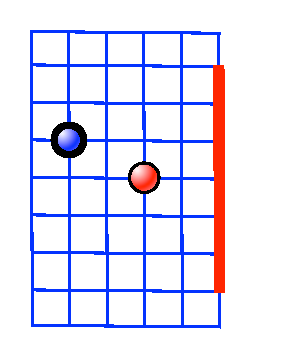
\includegraphics[width=130px]{images/save.pdf}
	\end{center}
\caption{Portiere in fase di parata del tiro avversario.}
\end{figure}

L'equazione per determinare il valore della parata \`e uguale a: $$ P_1 = \frac{agilit\grave{a}}{100} \cdot \frac{reattivit\grave{a}}{100} \cdot \left( 1-\frac{distanza}{diagonale} \right) $$ dove agilit\`a \`e il valore di agilit\`a del portiere espresso con un valore da 1 a 100, reattivit\`a \`e la velocit\`a di reazione, anch'essa espressa con un valore da 1 a 100, mentre l'ultimo coeffienciente \`e il risultato del rapporto inverso tra la distanza del portiere dal giocatore che sta effettuando il tiro e la diagonale del campo. \vspace{3mm}

La parata \`e in contrasto con il tiro visto nella sezione \ref{tiro}. Il tiro genera un valore che viene confrontato con quello generato dalla parata del portiere. In caso il valore $P_1$ sia inferiore a $T_1$, il portiere non \`e riuscito a parare il tiro (per merito dell'attaccante o demerito del portiere) e la palla \`e finita in rete. Nel caso in cui il valore $P_1$ sia uguale o maggiore di $T_1$ il portiere ha compiuto una parata e ha salvato la porta. \vspace{3mm}

L'azione ricomincia dal portiere con un passaggio verso un compagno per tentare un'azione d'attacco.

\subsubsection{Logica di Posizione}

Anche il portiere, in qualit\`a di giocatore come tutti gli altri, ha la possibilit\`a di gestire una situazione di ``emergenza'' rimanendo in posizione e non generando movimenti. Si faccia riferimento alla sezione \ref{posizione} per i dettagli della logica.

\newpage

\section{Modello}

Analizziamo ora il modello del sistema e la composizione delle classi e dei metodi principali necessari al corretto funzionamento del software come descritto nella tabella sottostante. \vspace{3mm}

\begin{table}[H]
\begin{center}
	\begin{tabular}{|l|l|l|}
		\hline
		\textbf{Classe} & \textbf{Identifica} & \textbf{Descrizione} \\ \hline \hline
		Timer & Tempo & Regola la durata del match e ne determina la fine. \\ \hline
		Field & Campo & Gestisce le dimensioni della superficie di gioco e il posizionamento \\
		& & di giocatori e palla su di esso. \\ \hline
		Referee & Arbitro & Controlla la regolarit\`a del gioco e fischia eventuali scorrettezze. \\ \hline
		Manager & Manager & Gestisce il modulo di gioco, effettua i cambi tra giocatori in \\
		& & campo ed in panchina e schiera la formazione d'attacco o di difesa. \\ \hline
		Team & Squadra & Associa i vari giocatori alla squadra di cui fanno parte. \\ \hline
		Player & Giocatore & Gioca la partita assieme ai compagni di squadra. \\ \hline
		Ball & Pallone & Oggetto condiviso dai giocatori \\ \hline
		\end{tabular}
\end{center}
\caption{La lista degli elementi principali che compongono il sistema.}
\end{table}

Le classi principali sono le 6 classi fondamentali appena presentate. Se mancasse anche solo una di esse, non si potrebbe realizzare il gioco nella nostra realt\`a virtuale. Ognuna di esse rappresenta un elemento presente e visibile nel campo di gioco ed attivamente partecipe allo svolgimento della partita. La sola eccezione vale per la classe \emph{Team} che si occupa di raggruppare i giocatori in un'unica squadra. \vspace{3mm}

\begin{figure}[H]
	\begin{center}
		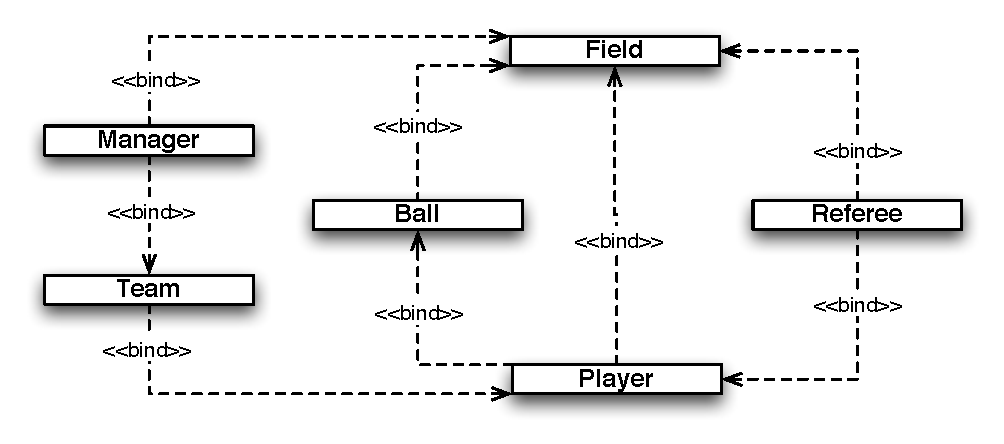
\includegraphics[width=400px]{images/relations-class-schema.pdf}
	\end{center}
\caption{Diagramma generale delle classi del sistema.}
\end{figure}

Lo schema esposto presenta le relazioni che intercorrono tra le classi principali del nostro gioco oltre all'indicazione del verso in cui la comunicazione \`e direzionata. \vspace{3mm}

Approfondiamo nelle prossime sezioni le singole classi entrando nel dettaglio per comprendere la loro tipologia e le funzioni principali che permettono il corretto svolgimento del gioco.

\subsection{Timer}

Il timer \`e la classe che si occupa della gestione del tempo. Ad intervalli regolari variabili incrementa un contatore che scandisce il trascorrere del tempo durante la partita. 

\begin{figure}[H]
	\begin{center}
		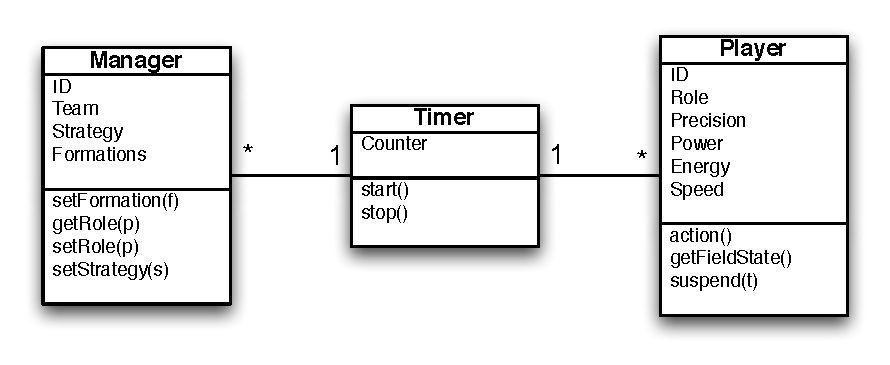
\includegraphics[width=350px]{images/timer-class.pdf}
	\end{center}
\caption{Diagramma delle classi per il timer di gioco.}
\end{figure}

La classe tempo ha metodi di accesso diretto a tutti i processi attivi in campo che necessitanto una inizializzazione simultanea ovvero:

\begin{itemize}
	\item giocatori
	\item manager
	\item arbitro
\end{itemize}

In questa maniera il gioco inizia simultaneamente per tutte le parti coinvolte che cominciano ad interagire tra di loro e con gli oggetti passivi. Al termine della partita, per lo stesso principio, un metodo della classe si occupa di mettere in stop i thread decretando il termine della partita e l'eventuale vincitore se non si verifica una situazione di parit\`a.

\subsection{Campo}

Il campo deve essere la classe di riferimento necessariamente accessibile a tutti i giocatori in campo. Si occupa di salvare i posizionamenti dei giocatori nell'area di gioco a seguito dei movimenti effettuati e di fornire alcune informazioni legate al campo di gioco come ad esempio la posizione del pallone e la dislocazione delle porte. \vspace{3mm}

Ad ogni giocatore che effettua l'interrogazione di stato restituisce:

\begin{itemize}
	\item la posizione nel campo di gioco;
	\item le direzioni percorribili;
	\item la posizione dei compagni;
	\item la posizione degli avversari;
	\item la posizione del pallone;
\end{itemize}

Ogni giocatore deve poter accedere alla classe \emph{Field}, effettuare la richiesta del vettore delle posizioni ed attendere una risposta dalla classe. Essa restitur\`a una lista contenente le informazioni relative alla posizione dei compagni, degli avversari e del pallone necessarie al giocatore per poter compiere il proprio movimento in gioco coerentemente con gli spazi disponibili e con la logica applicata. \vspace{3mm}

\begin{figure}[H]
	\begin{center}
		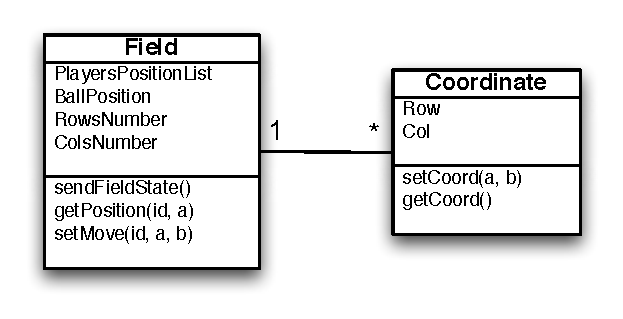
\includegraphics[width=220px]{images/field-class.pdf}
	\end{center}
\caption{Diagramma delle classi per il campo di gioco.}
\end{figure}

I valori delle dimensioni di gioco e delle aree di movimento sono inizializzate non appena vengono definite la tipologia di partita (calcio/calcetto) e il numero di giocatori in campo. \vspace{3mm} 

Un vettore di posizioni contiene i vari posizionamenti dei giocatori e lo schieramento a cui appartengono. Una variabile ad-hoc contiene invece il posizionamento del pallone e viene trattato in modo similare al vettore precedente. \vspace{3mm}

Le funzioni che permettono di accedere ai vettori di stato sono:

\begin{description}
	\item[function GetPositions return PositionList] che ritorna un listato di posizioni dei vari giocatori in campo;
	\item[function GetBallPosition return Position] che restituisce la posizione della palla in campo;
\end{description}

Nel caso si trovi al limite della propria area di movimento, le uniche azioni possibili sono: rimanere nella propria posizione e non compiere alcun movmento o, in alternativa, muovere lateralmente per avvicinarsi al giocatore con la palla (se visibile). \vspace{3mm}

Il campo gestisce anche alcuni eventi particolari legati all'uscita del pallone dall'area di gioco. Mentre possiamo ammettere che un giocatore rimanga tutta la partita in campo e quando raggiunga il bordo del campo non possa attraversarlo, \`e lecito pensare che il pallone fuoriesca dall'area di gioco. In questo caso viene lanciata una eccezione e la palla passa alla squadra avversaria. Si possono verificare 3 casi principali:

\begin{description}
	\item[Fallo laterale] avviene quando un giocatore lancia la palla oltre la linea laterale del campo. La palla passa ad un giocatore avversario e il gioco riprende dal bordo in cui \`e avvenuta l'uscita, punto in cui vengono riposizionati giocatore e pallone; 
	\item[Rimessa dal fondo] \`e causata da un giocatore avversario che scaglia la palla oltre la linea della porta aversaria. Il pallone passa al portiere e il gioco ricomincia dal fondo del campo;
	\item[Calcio d'angolo] viene fischiato quando un giocatore lancia la palla oltre la linea della propria porta. Il gioco riprende dall'angolo con il riposizionamento di palla e giocatore;
\end{description}

La funzione che permette all'arbitro di resettare le posizioni in base all'evento \`e:

\begin{description}
	\item[procedure ResetPosition(ID : in Integer; P : Position)] nella quale viene passata l'ID del giocatore che andr\`a a battere la rimessa e la posizione in cui verranno posizionati giocatore e pallone;
\end{description}

\subsection{Arbitro}
\label{arbitro}

L'arbitro \`e di per se un'entit\`a molto semplice: non \`e presente direttamente nel campo di gioco e viene richiamato in casi chiaramente definiti per determinare il corretto svolgimento del gioco. \vspace{3mm}

Le casistiche in cui l'arbitro viene chiamato in causa sono:

\begin{itemize}
	\item contrasto tra due giocatori (possibile fallo);
	\item palla oltre il limite del campo:
	\begin{itemize}
		\item fallo laterale;
		\item rimessa dal fondo;
		\item calcio d'angolo;
	\end{itemize}
	\item fuorigioco (non trattato);
\end{itemize}

In tutti i casi, il fischio dell'arbitro comporta il fermo del gioco, la riassegnazione della palla e l'inizio di una nuova azione. \vspace{3mm}

Definiamo cosa fa l'arbitro nei casi sopra esposti:

\begin{itemize}
	\item fallo tra giocatori:
	\begin{enumerate}
		\item mantiene la posizione della palla sul punto del fallo;
		\item mantiene la posizione del giocatore che ha subito il fallo vicino alla palla;
		\item riposiziona posiziona l'altro giocatore a distanza definita;
		\item fa riprendere il gioco;
	\end{enumerate}
	\item palla fuori dal campo:
	\begin{enumerate}
		\item posiziona la palla sul bordo del campo nel punto di uscita;
		\item posiziona il giocatore sulla palla;
		\item ne assegna il possesso;
		\item fa riprendere il gioco;
	\end{enumerate}
\end{itemize}

Nello schema sottostante si comprende facilmente come l'arbitro intervenga nelle varie fasi di gioco ed interagisca con le altre classi.

\begin{figure}[H]
	\begin{center}
		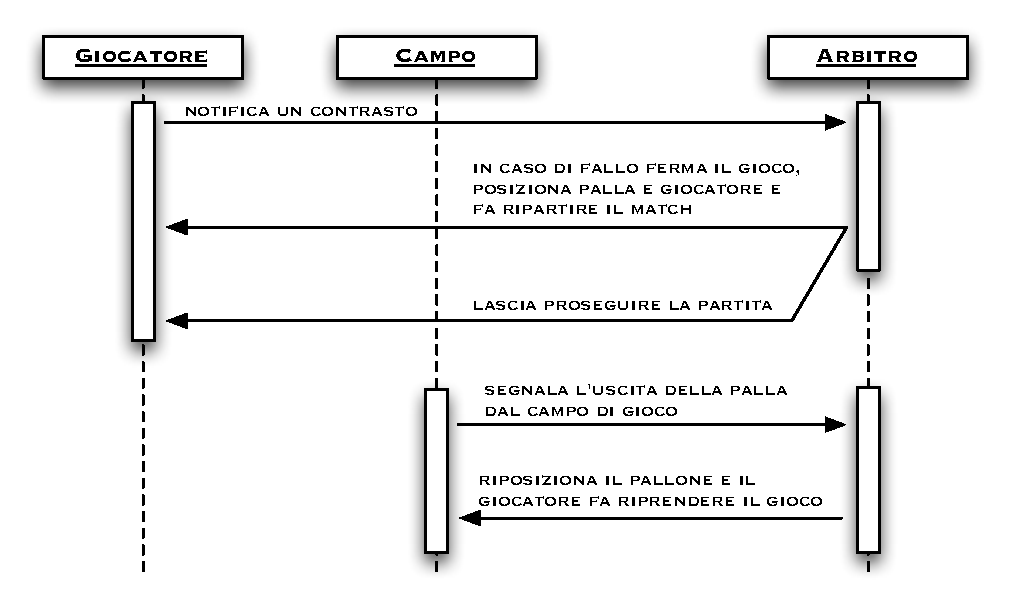
\includegraphics[width=400px]{images/referee-sequence.pdf}
	\end{center}
\caption{Diagramma di sequenza dell'arbitro di gioco.}
\end{figure}

L'unico aspetto determinante rispetto a quanto visto sotto \`e legato esclusivamente alla priorit\`a con cui l'arbitro interviene nel gioco: per un'analisi dettagliata delle priorit\`a in campo, rimandiamo alla sezione \ref{priorita} in cui vengono trattate nello specifico.

\subsection{Manager}
\label{manager}

Il Manager deve essere considerato la mente del gioco in quanto non partecipa attivamente alla partita ma si occupa di definire le strategie di gioco e i cambi tra giocatori in campo o in panchina. Le scelte legate alla posizione dei giocatori e alle strategie sono legate ad alcuni fattori oggettivi che permettono al manager di prendere le decisioni opportune per modificare la squadra in campo:

\begin{itemize}
	\item risultato parziale della partita;
	\item numero di giocatori in campo (a seguito di potenziali espulsioni o infortuni);
	\item sbilanciamento attuale della formazione (attacco o difesa);
	\item formazione in campo;
	\item modulo di gioco;
\end{itemize}

Manager \`e un thread che viene risvegliato ad intervalli regolari per visionare e comprendere l'andamento del match ed apportare correzioni alla squadra oppure in casi particolari in cui viene risvegliato. Gli eventi che scatenano il Manager possono essere identificati da:

\begin{itemize}
	\item gol della propria squadra;
	\item gol della squadra avversaria;
	\item energia di un giocatore che scende sotto una soglia predefinita (e necessita un cambio);
	\item giocatore che subisce un infortunio durante la partita;
	\item fischio dell'arbitro per contrasto tra giocatori;
	\item espulsione di un giocatore in campo;
\end{itemize}

\begin{figure}[H]
	\begin{center}
		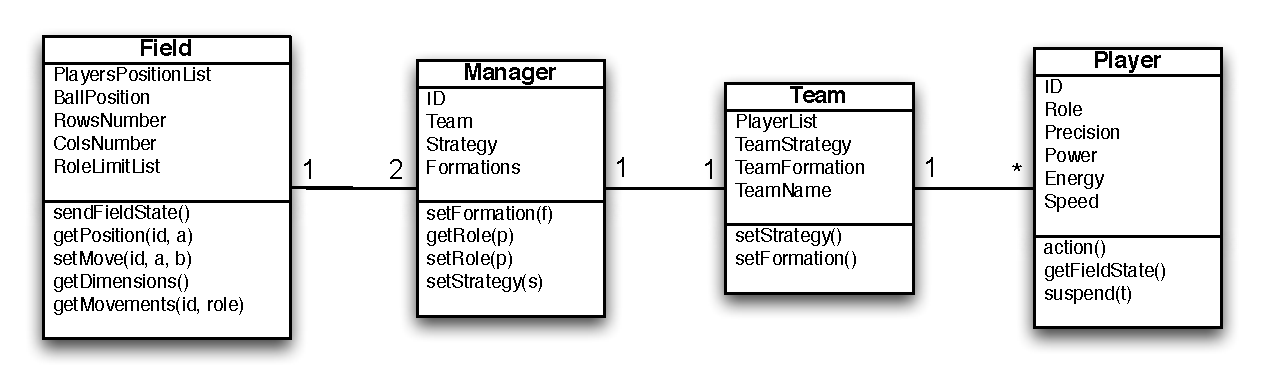
\includegraphics[width=440px]{images/manager-class.pdf}
	\end{center}
\caption{Diagramma delle classi per il manager della squadra.}
\end{figure}

Come descritto nel diagramma sopra esposto, il manager ha una relazione diretta con i giocatori attraverso la classe \emph{Team}'' con la quale pu\`o visionare lo stato dell'affaticamento ed eventuali ulteriori caratteristiche proprie di ogni singolo elemento. Inoltre \`e direttamente collegato con la classe squadra che raggruppa tutti i giocatori per apportare eventuali variazioni a cui \`e soggetta tutta la squadra piuttosto che un singolo giocatore specifico. \vspace{3mm}

Pu\`o inoltre accedere alla classe \emph{Field} che gli permette di conoscere il posizionamento dei giocatori in campo nonch\`e quello della palla attraverso la funzione \emph{getFieldState()}, uguale a quella utilizzata dai giocatori. Anche questi fattori sono determinanti al fine di prendere decisioni per la propria squadra. \vspace{3mm}

A seguito dei risultati della propria elaborazione, possono essere effettuati interventi come:

\begin{itemize}
	\item cambio di formazione;
	\item sostituzione di un giocatore;
	\item cambio di posizione tra giocatori in campo;
	\item cambio della propensione di gioco (attacco/difesa);
\end{itemize}

Nel diagramma sottostante invece viene analizzato lo schema di comunicazione degli stati da parte del Manager che, come gi\`a visto, interroga il campo e i giocatori per ottenere il quadro della situazione per effettuare le variazioni necessarie. \vspace{3mm}

\begin{figure}[H]
	\begin{center}
		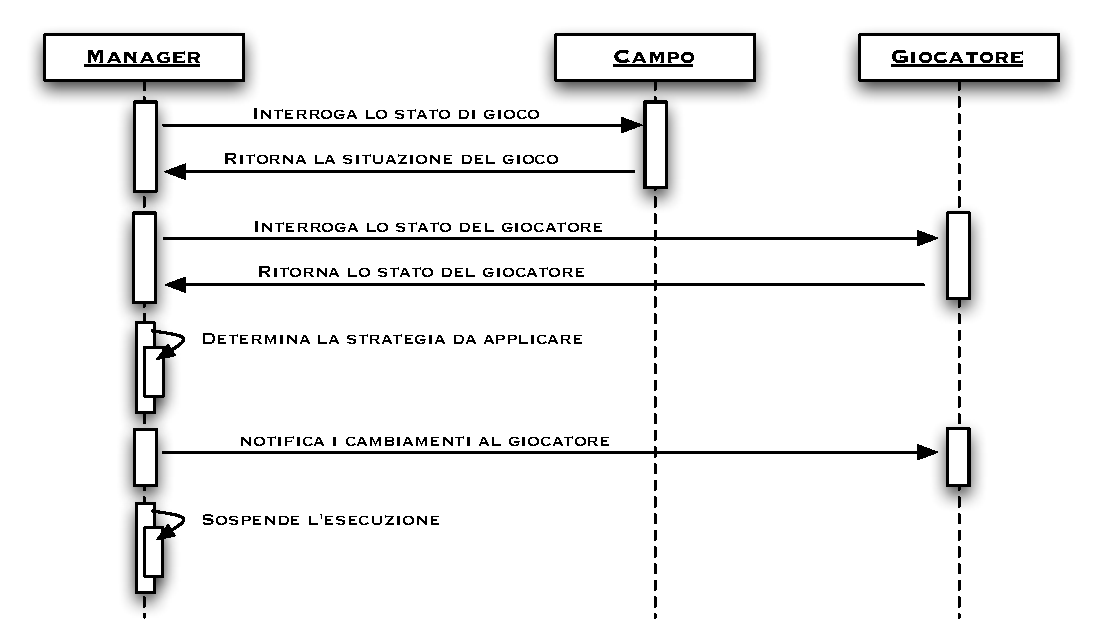
\includegraphics[width=400px]{images/manager-sequence.pdf}
	\end{center}
\caption{Diagramma di sequenza del manager.}
\end{figure}

Anche il Manager deve avere una priorit\`a differente rispetto a quella dei giocatori in campo. Rimandiamo alla sezione \ref{priorita} per ulteriori chiarimenti.

\subsection{Squadra}
\label{squadra}

La classe squadra \`e una classe molto semplice nella nostra realt\`a di gioco. \`E l'elemento che funge da contenitore per i giocatori e che permette di raggrupparli in due insiemi differenti. \vspace{3mm}

La classe squadra permette di facilitare il coordinamento dei giocatori, la diffusione di alcune specifiche impartite dal Manager a tutti i giocatori della squadra in campo e non soltanto a qualche istanza di giocatore particolare. Il modulo in campo e lo sbilanciamento della squadra in attacco o in difesa sono caratteristiche generali e l'oggetto di riferimento \`e la classe squadra, piuttosto che tutti i singoli giocatori che le appartengono. \vspace{3mm}

I metodi principali appartenenti alla classe \emph{Team} sono:

\begin{description}
	\item[procedure SetStrategy(S : in Strategy)] che imposta la strategia di gioco;
	\item[procedure SetModule(M : in Module)] che setta il modulo di gioco;
	\item[function GetStrategy return Strategy] restituisce ai giocatori ed al manager la strategia applicata;
	\item[function GetModule return Module] restituisce ai giocatori ed al manager il modulo di gioco in uso;
\end{description}

\begin{figure}[H]
	\begin{center}
		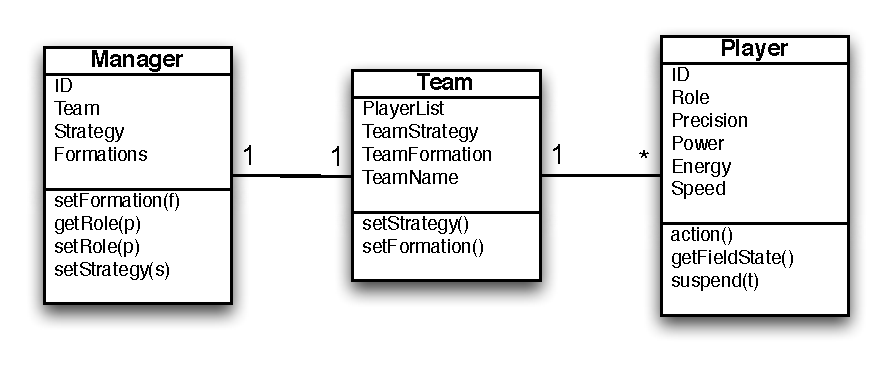
\includegraphics[width=340px]{images/team-class.pdf}
	\end{center}
\caption{Diagramma delle classi per la classe squadra.}
\end{figure}

Manager \`e l'unica entit\`a in grado di accedere direttamente alla squadra ed effettuare variazione. I giocatori subiscono tali modifiche in riferimento alla classe squadra di cui fanno parte e leggono le modifiche apportate attraverso i comandi \emph{Get}.

\subsection{Giocatore}
\label{giocatore}

I giocatori sono i task di base necessari per lo svolgimento del gioco e vengono intesi come multiple istanze dello stesso task. \vspace{3mm}

Ognuno di essi \`e contraddistinto da una serie di caratteristiche proprie e legate al ruolo, alla posizione e alle abilit\`a:

\begin{itemize}
	\item \textbf{ID:} ogni giocatore possiede un ID univoco generale che permette di identificare il processo rispetto tra tutti gli altri processi giocatore in campo al fine di determinare il possessore della risorsa condivisa o identificarne nel vettore delle posizioni in campo;
	\item \textbf{Ruolo:} determina il posizionamento in campo e le possibilit\`a di movimento all'interno dell'area specifica di gioco.
	\item \textbf{Visibilit\`a:} \`e il parametro che determina l'abilit\`a di visione del gioco di ogni singolo giocatore.
	\item \textbf{Potenza:} \`e il parametro che determina la potenza di tiro e di contrasto del giocatore. \`E un valore tra 0 e 100.
	\item \textbf{Precisione:} contraddistingue l'abilit\`a del giocatore in questione nel giostrare il pallone.
	\item \textbf{Velocit\`a:} identifica la velocit\`a del giocatore ovvero la quantit\`a di movimenti che pu\`o compiere rispetto ad altri.
	\item \textbf{Energia:} rappresenta la resistenza del giocatore durante la partita. \`E un parametro che decrementa (in modo lineare o esponenziale) con il proseguire delle azioni di gioco fino alla fine della partita.
\end{itemize}

Ogni giocatore \`e definito da un processo che compie in maniera ciclica tre azioni base:

\begin{itemize}
	\item \textbf{getFieldState():} il giocatore apprende lo stato del gioco ed in particolare il posizionamento dei compagni, degli avversari e della palla;
	\item \textbf{action():} sulla base dello stato del gioco e limitatamente alla propria visibilit\`a, ogni giocatore effettua una mossa tra quelle definite nelle logiche di gioco a disposizione;
	\item \textbf{suspend():} al termine dell'azione, ogni giocatore sospende la propria esecuzione per un tempo definito. Al termine dell'attesa procede con una nuova azione;
\end{itemize}

Il diagramma esposto identifica quali sia la sequenza delle azioni che ogni giocatore compie durante la propria fare di gioco. Inizialmente procede con una interrogazione del campo al fine di ottenere lo stato del gioco. Il campo risponde con un vettore contenente i posizionamenti dei vari giocatori in campo nonch\`e quella del pallone. Segue immediatamente una fase di analisi dell'area ``visibile'' al fine di determinare quale sia l'azione ottimale da compiere. L'azione viene portata a termine e viene inviato al campo il posizionamento del giocatore a seguito della manovra effettuata. Dopo la notifica, il processo si sospende per un tempo \emph{t} noto al fine di lasciare agli altri processi gicatore la possibilit\`a di operare a loro volta.

\begin{figure}[H]
	\begin{center}
		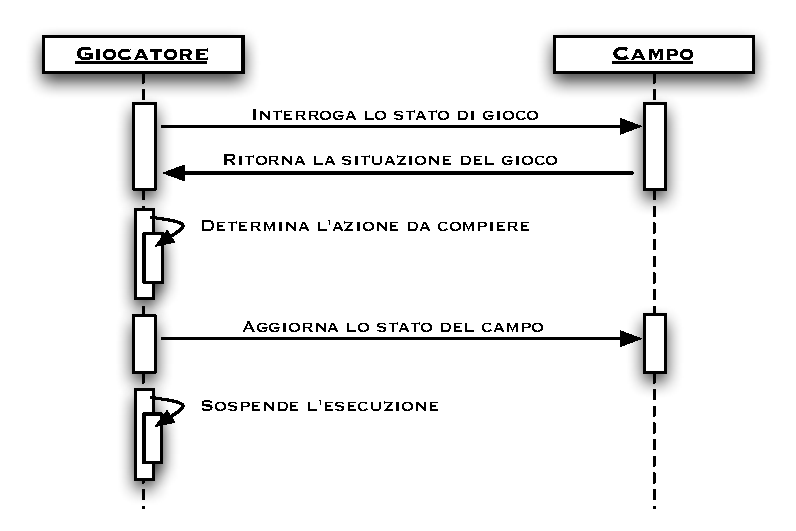
\includegraphics[width=300px]{images/sequence-player.pdf}
	\end{center}
\caption{Diagramma di sequenza del giocatore.}
\end{figure}

Il diagramma degli stati presenta in forma semplificata i vari stadi in cui il giocatore si pu\`o trovare in ogni istante di tempo. \vspace{3mm}

\begin{figure}[H]
	\begin{center}
		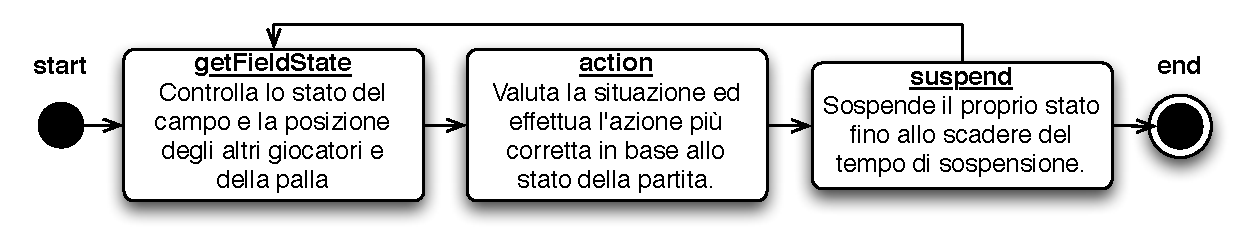
\includegraphics[width=400px]{images/player-state.pdf}
	\end{center}
\caption{Diagramma di stato dei giocatori in campo.}
\end{figure}

La parte pi\`u consistente del processo \`e tutta contenuta nello stato \emph{action}, il quale si occupa di valutare le posizioni ed applicare la logica opportuna. Lo schema che segue indica dettagliatamente, passo per passo, tutte le funzioni che vengono applicate per creare il quadrato visibile al giocatore al fine di consentirgli il passaggio ad altri compagni o movimenti in una delle quattro direzioni possibili. All'interno dello schema esistono due diramazioni, legate alla possibilit\`a che il giocatore detenga o meno il possesso di palla oppure che la squadra sia in possesso di palla attraverso un compagno. Nel caso entrambi i test siano negativi, prendiamo come regola che gli avversari siano in possesso del pallone, senza applicare ulteriori test.

\begin{figure}[H]
	\begin{center}
		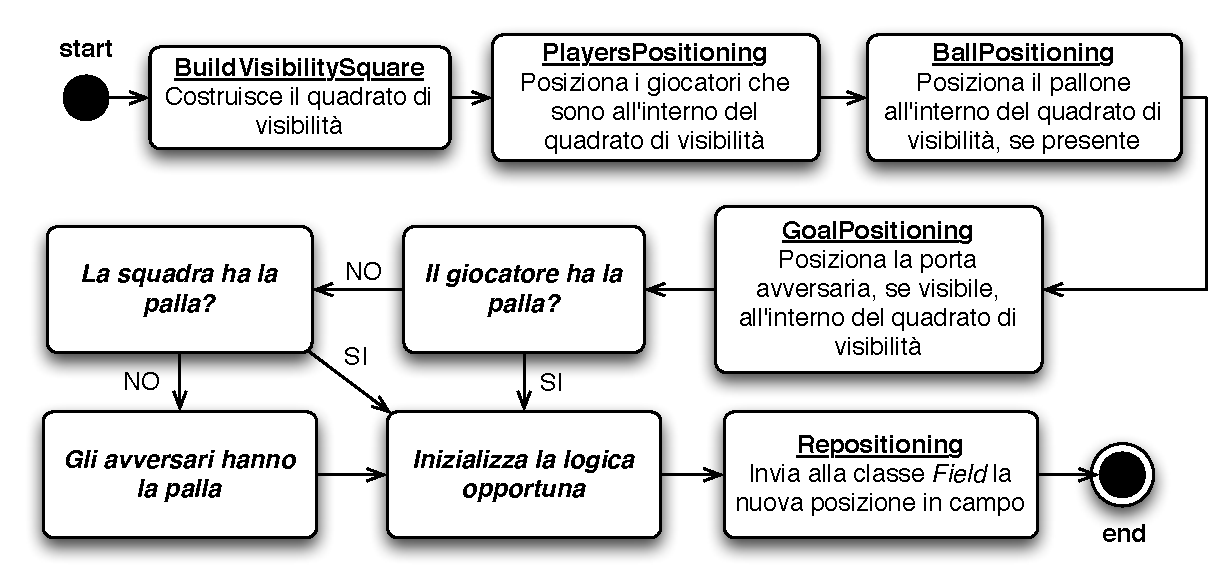
\includegraphics[width=400px]{images/player-action.pdf}
	\end{center}
\caption{Diagramma dell'azione di gioco del giocatore.}
\end{figure}

Un'ulteriore caratteristica che diversifica il gioco \`e la possibilià di impostare per ogni singolo giocatore tempi di \emph{suspend} differenti attraverso la valorizzazione del relativo parametro. Il risultato ottenuto è così quello di avere tempo di reazione differenti legati alla dimensione del tempo di sospensione. Giocatori più reattivi possiederanno tempi di sospensione più bassi. Al contrario, giocatori più lenti avranno parametri via via più elevati fino ad un limite ragionevole. \vspace{3mm}

Andiamo ad analizzare infine la situazione della memoria e della CPU durante il gioco nel diagramma di Garrett esposto. Ogni giocatore comincia la partita in una coda di processi pronti. Nel primo istante utile, un processo prende possesso della CPU e compie le azioni viste precedentemente fino allo scadere del tempo di utilizzo del processore o fino alla sospensione. Una volta sospeso, entra in un'altra coda, quella dei processi sospesi, e attende il termine del tempo di sospensione \emph{t}. Una volta pronto, passa nuovamente nella coda dei processi pronti per procedere con una nuova azione non appena avr\`a a disposizione la CPU.

\begin{figure}[H]
	\begin{center}
		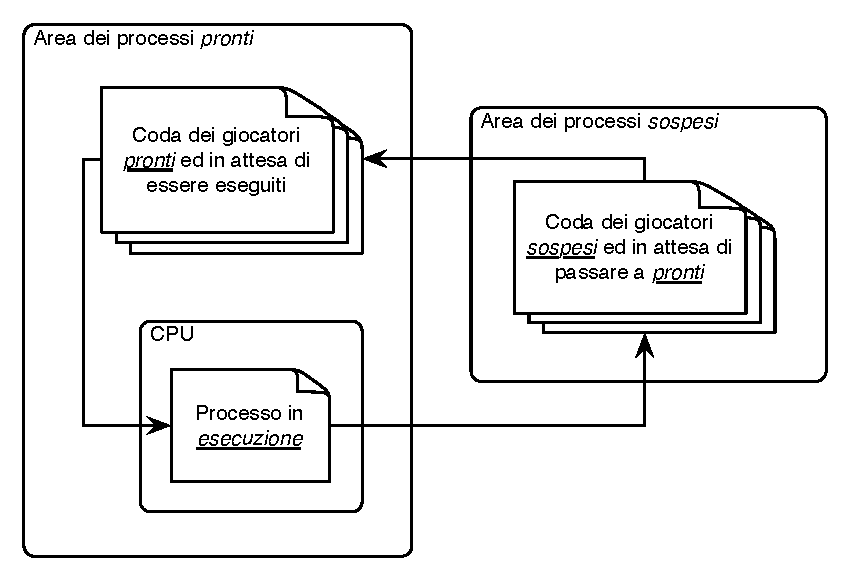
\includegraphics[width=300px]{images/player-schema.pdf}
	\end{center}
\caption{Diagramma di stato dei giocatori in campo.}
\end{figure}

\subsection{Pallone}
\label{pallone}

Il pallone rappresenta la risorsa condivisa nel campo di gioco. Ogni giocatore concorre per ottenerne il possesso e poter condurre la palla nella rete avversaria e segnare un gol in favore della propria squadra. \vspace{3mm}

Il pallone \`e rappresentato nel campo come una risorsa condivisa il cui accesso da parte dei giocatori \`e limitato e regolato da un monitor. Ci\`o preclude la possibilit\`a che la palla possa essere in possesso di pi\`u di un giocatore contemporaneamente. Ada 95 mette a disposizione il costrutto \emph{protected type} che si occupa di costruire e gestire i monitor per l'accesso in mutua esclusione alla risorsa. \vspace{3mm}

Dal punto di vista logico possiamo immaginare il pallone come un oggetto sul campo di gioco il quale viene spostato dai giocatori attraverso avanzamenti con palla, passaggi, tiri in porta o contrasti. Dal punto di vista tecnico, si tratta di un'entit\`a passiva che ``subisce'' le azioni che vengono compiute su di esso da parte dei giocatori. \vspace{3mm}

In questo caso la classe si riduce ad un oggetto protetto con pochi metodi accessibili per ottenere la sua posizione, l'eventuale possessore, effettuare un movimento della sfera in una delle 4 direzioni o eventualmente settarne il possessore. \vspace{3mm}

La risorsa protetta contiene una variabile fondamentale che permette di identificare il thread che ne detiene il possesso. In questa maniera, anche nel caso in cui il giocatore possessore della palla entri in stato di \emph{sleep}, una guardia garantir\`a che nessun altro dei 21 giocatori rimanenti possa accedere alla risorsa. \vspace{3mm}

\begin{figure}[H]
	\begin{center}
		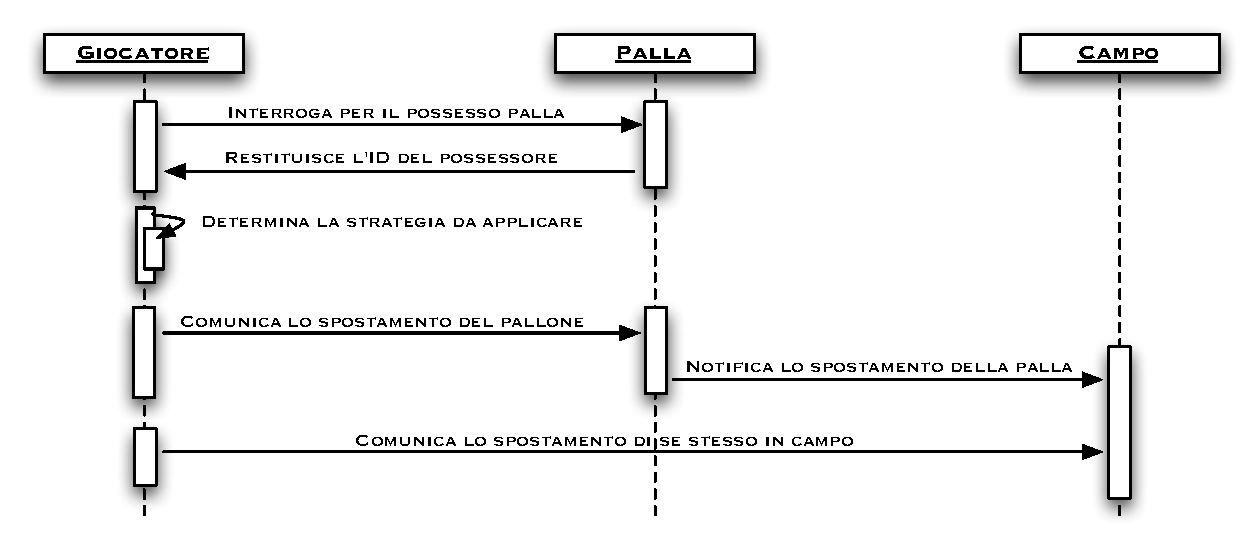
\includegraphics[width=440px]{images/ball-movement.pdf}
	\end{center}
\caption{Diagramma di sequenza dello spostamento della palla in campo.}
\end{figure}

Al fine di gestire il movimento della palla \`e stato creato un thread apposito \emph{TaskBall} che si occupa di rilevare e gestire il movimento del pallone

Per maggiori dettagli sui metodi legati alla risorsa protetta rimandiamo alla sezione \ref{possessopalla} in cui vengono analizzati gli aspetti relativi alla concorrenza per un oggetto condiviso.

\newpage

\section{Concorrenza}
\label{concorrenza}

Prima di entrare nel dettaglio dei problemi legati alla concorrenza, cerchiamo di identificare chiaramente quali sono le entit\`a che fanno parte del nostro gioco e come interagiscano al fine di un corretto funzionamento:

\begin{description}
	\item[Entit\`a Attive:] rappresentate dai giocatori in campo, dal manager che li dirige e dall'arbitro come direttore di gara. Sono i thread attivi che compiono movimenti sul campo secondo scelte determinate in base alla situazione che rilevano nel momento in cui vengono attivati. Lo stesso vale per i manager che rivedono posizioni e formazione in campo in base al risultato e all'andamento della gara. L'arbitro monitora lo stato di gioco e, in base a determinati eventi, decide l'andamento della gara attraverso modifiche allo stato di gioco.
	\item[Entit\`a Reattiva:] identificata dal pallone e dal campo di gioco. Rappresentano entit\`a che non hanno potere decisionale, ma subiscono variazioni sulla base dell'intervento dei giocatori che ne hanno via via il possesso. Il pallone pu\`o muovere assieme al giocatore in caso di avanzamento con palla o in maniera autonoma nei casi di passaggio o tiro in porta. Il movimento della palla \`e comunque sempre subordinato alla potenza impressagli dal giocatore che effettua l'azione. Il campo subisce tutte queste variazioni e si occupa di mantenere uno stato di gioco consistente.
\end{description}

Le situazioni di concorrenza che dobbiamo necessariamente analizzare e risolvere al fine di perfezionare il gioco ed eliminare situazioni impreviste sono fondamentalmente:

\begin{itemize}
	\item integrit\`a dello stato di gioco;
	\item unicit\`a del possesso di palla;
	\item prevenzione di situazioni di stallo;
\end{itemize}

Esaminiamo perci\`o ognuna di esse e forniamo gli elementi necessari per la loro risoluzione.

\subsection{Integrit\`a dello Stato di Gioco}
\label{statodigioco}

Avere 22 processi che modificano costantemente lo stato del campo di gioco in un ciclo di durata pari al tempo totale di gioco pu\`o causare facilmente seri problemi di inconsistenza a livello di campo di gioco. In questo senso \`e necessario prevedere tale situazione ed utilizzare tecniche di programmazione che permettano di evitarla per poter procedere sempre correttamente con l'aggiornamento dello stato e dare la possibilit\`a ai thread che lo necessitano, di conoscere la condizione di gioco. \vspace{3mm}

Le strade percorribili sono fondamentalmente due:
\begin{enumerate}
	\item instanziare la classe \emph{Field} come processo;
	\item creare la classe \emph{Field} come tipo protetto;
\end{enumerate}

La prima soluzione, pi\`u simile ad una struttura di tipo client/server, garantisce attraverso l'utilizzo di una struttura di tipo \emph{select} a cui fanno seguito una serie di \emph{accept} legate alla scrittura e alla lettura, accesso esclusivo al thread che gestisce i posizionamenti nel campo. La soluzione \`e percorribile se immaginiamo di istanziare su macchine differenti i giocatori e il thread del campo di gioco. \vspace{3mm}

Diventa perci\`o pi\`u semplice gestire la classe \emph{Field} come un tipo protetto che garantisce la mutua esclusione delle operazioni che intervengono sulla classe, mantenendo pertanto la correttezza dello stato di gioco attraverso la gestione da parte del linguaggio degli accessi alle variabili protette. La soluzione non impatta direttamente sul processore in quanto la CPU non viene occupata direttamente dalla classe \emph{Field} ma dai thread dei giocatori che vi devono accedere. \vspace{3mm}

La classe \emph{Field} \`e pertanto dotata dei metodi: \vspace{3mm}

\begin{description}
	\item[function GetPositions return PositionList] che permette di interrogare il campo ed ottenere il vettore contenente le posizioni di tutti i giocatori nell'area di gioco, compresa quella del giocatore interrogante. La funzione, come specifica del linguaggio Ada 95, ha come prerogativa l'accesso ai dati in sola lettura, evitando la modifica del campo di gioco. Questo permette l'accesso concorrente in \emph{read only} al vettore delle posizioni;
	\item[procedure SetPosition(ID : in Integer; M : in Move)] da la possibilit\`a al giocatore che lancia la procedura di modificare la propria posizione nel campo di gioco, indicando il proprio ID univoco e la tipologia di movimento come da specifiche gi\`a trattate nella sezione \ref{movimento}. In questo modo viene aggiornata la posizione nel vettore senza incorrere in problemi di inconsistenza;
	\item[function GetBallPosition return Position] permette al giocatore di conoscere la posizione della palla all'interno del campo di gioco. \`E necessaria al fine di permettere al processo di decidere quale azione compiere, limitatamente alla propria visibilit\`a di gioco;
\end{description}

Queste tre funzioni da sole permettono di ottenere tutte le informazioni necessarie al corretto svolgimento del gioco non solo per i thread giocatori, ma anche eventualmente a manager ed arbitri per effettuare decisioni o correzioni durante lo svolgimento della partita. La garanzia di mutua esclusione \`e determinata dalla stessa classe \emph{Field} in quanto dichiarata come risorsa protetta ad accesso limitato.

\begin{figure}[H]
	\begin{center}
		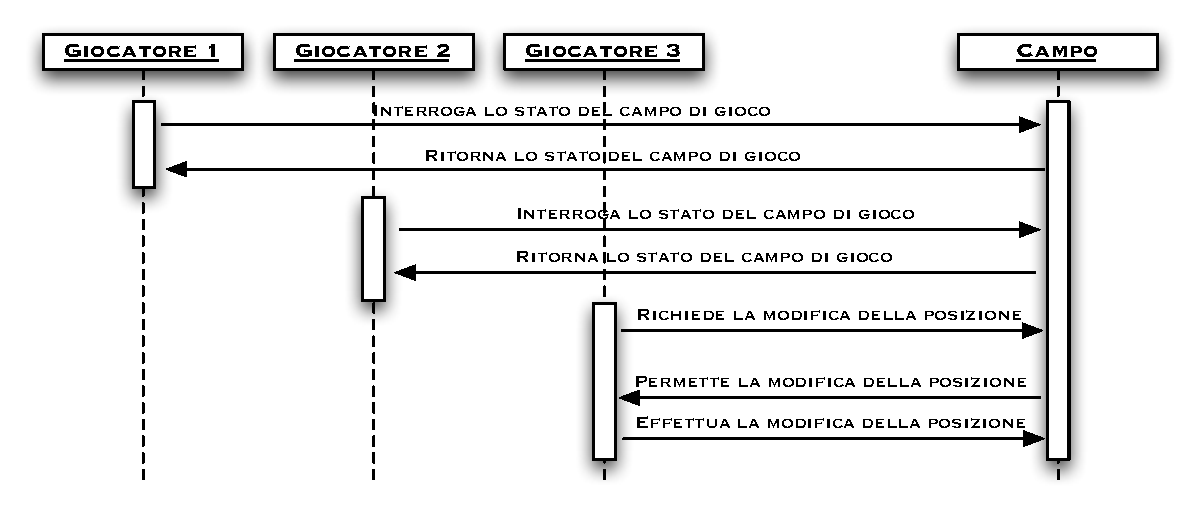
\includegraphics[width=440px]{images/concurrent-game-state.pdf}
	\end{center}
\caption{Diagramma di sequenza delle richieste dei giocatori per la notifica e la modifica delle posizioni.}
\end{figure}

Nello schema sopra esposto \`e possibile notare come la lettura delle posizioni in campo sia un processo di lettura concorrente, mentre l'aggiornamento della posizione del giocatore sia un'operazione esclusiva. In questo senso, una volta terminate le eventuali operazioni di lettura, il processo prende il controllo della risorsa, effettua il cambiamento e la rilascia. \vspace{3mm}

\subsection{Unicit\`a del Possesso di Palla}
\label{possessopalla}

Un altro problema evidente legato alla concorrenza tra thread \`e quello del possesso palla da parte dei giocatori in campo. Il pallone risulta l'unica istanza esistente e non \`e realistico, nella nostra realt\`a virtuale cos\`i come nella realt\`a di gioco vero e proprio, la condizione in cui due giocatori distinti detengano contemporaneamente il possesso del pallone. \vspace{3mm}

Si rende pertanto necessario l'utilizzo di un meccanismo che garantisca il mutuo accesso alla risorsa. Anche in questo senso Ada 95 ci viene incontro fornendo uno strumento per la gestione delle risorse protette. Dichiarando la palla come risorsa protetta, garantiamo l'accesso esclusivo ai dati in essa contenuti. \vspace{3mm}

I metodi utilizzabili con la classe palla sono:

\begin{description}
	\item[function GetOwner return Integer] permette di ottenere l'ID dell'attuale possessore del pallone o il valore \emph{null} nel momento in cui non esistesse in quell'istante un possessore della risorsa;
	\item[function GetBallPosition return Position] ritorna la coordinata relativa alla posizione del pallone con lo scopo di prenderne possesso nel caso si trovi in intersezioni adiacenti a quella del giocatore che sta effettuando la richiesta;
	\item[procedure SetOwner(ID : in Integer)] \`e forse il metodo principale della classe. Esso permette di settare il valore della variabile relativa al proprietario della risorsa. Essendo una procedura, garantisce la mutua esclusione nell'attivit\`a attraverso il meccanismo implicito del monitor, impedendo che un giocatore, una volta flaggato il \emph{lock} sulla risorsa, non possa settare il proprio valore ID nella variabile a causa di una sospensione. Una situazione di questo genere porterebbe ad un'evidente inconsistenza di sistema, causando l'impossibilit\`a di accedere alla risorsa da parte di tutti gli altri giocatori per tutta la durata del match;
	\item[procedure KickBall(M : in Move; P : in Interger)] rappresenta la liberazione della risorsa attraverso un ideale ``calcio''. In questa procedura, anch'essa atomica ed indivisibile, il giocatore rimuove il blocco sulla risorsa settando la variabile a \emph{null} e applica una potenza al colpo in una direzione determinata;
\end{description}

Come abbiamo avuto modo di esaminare per la classe \emph{Field}, i metodi appena visti garantiscono accesso esclusivo alla risorsa per eventuali modifiche al suo stato interno, mentre garantiscono accesso concorrente alle informazioni, permettendo a tutti i giocatori di identificarne proprietario e posizione, ma assicurando l'integrit\`a della risorsa.

\subsection{Priorit\`a dei Processi}
\label{priorita}

Al fine di gestire il corretto andamento del gioco, \`e necessario gestire le priorit\`a dei thread. Se cos\`i non fosse, ognuno di essi entrerebbe nella coda dei pronti e dovrebbe attendere diversi cicli di CPU prima di poter eseguire. Per questo motivo \`e necessario raggruppare le tipologie di processi e ordinarle seguendo una logica prioritaria d'esecuzione. \vspace{3mm}

I processi pi\`u comuni sono quelli dei giocatori in campo. Tutti i giocatori eseguono con la stessa priorit\`a, attraverso una politica di ordinamento di tipo ``FIFOWithinPriorities'', demandando eventuali gestioni ulteriori allo scheduler di sistema che li tratter\`a come processi ordinari. \vspace{3mm}

Con priorit\`a maggiore intervengono i manager delle squadre che, una volta pronti, devono entrare in esecuzione prima dei giocatori in stato di pronto, al fine di modificare le condizioni di gioco preventivamente rispetto al successivo intervento dei giocatori che dovranno gi\`a riscontrare la situazione variata. \vspace{3mm}

Infine l'arbitro, in qualit\`a di giudice di gioco deve poter intervenire immediatamente interrompendo il gioco, effettuando eventuali riposizionamenti di giocatori e di palla, prima di ogni giocatore e ancor prima delle decisioni dei manager.

\begin{table}[H]
\begin{center}
	\begin{tabular}{l l l }
		\hline
		\textbf{Classe} & \textbf{Priorit\`a} & \textbf{Descrizione} \\ \hline \hline
		Giocatore & 1 & Priorit\`a minima di accesso alla CPU. \\ \hline
		Manager & 2 & Priorit\`a superiore a quella dei giocatori. \\ \hline
		Arbitro & 3 & Priorit\`a massima. \\ \hline
	\end{tabular}
\end{center}
\caption{La lista delle priorit\`a dei processi.}
\end{table}

In particolare, poich\`e l'arbitro reagisce a situazioni che ne richiamano l'attenzione in maniera del tutto similare ad una ``entit\`a reattiva''

In questo modo viene garantito il corretto accesso al processore ed eventuali modifiche che devono essere applicate al gioco vengono recepite immediatamente da tutti i processi con priorit\`a inferiore per effetto del'ordine di esecuzione.

\subsection{Prevenzione delle Situazioni di Stallo}
\label{stallo}

Avere un numero elevato di processi che concorrono ad un'unica risorsa pu\`o portare facilmente a situazioni di stallo. Elenchiamo per completezza le tre situazioni in cui il sistema non \`e in grado di procedere oltre determinando una partita infinita o immodificabile fino alla fine del tempo di gioco:

\begin{itemize}
	\item deadlock;
	\item starvation;
	\item lockout;
\end{itemize}

Per non incappare nelle situazioni di cui sopra \`e necessario risolvere una o pi\`u tra le precondizioni elencate:

\begin{description}
	\item[Mutua esclusione:] non pi\`u di un processo alla volta ha accesso alla risorsa condivisa;
	\item[Cumulazione di risorse:] i procesi possono accumulare risorse e trattenerle mentre attendono di acquisirne altre;
	\item[Assenza di prerilascio:] le risorse vengono rilasciate solo volontariamente;
	\item[Attesa circolare:] un processo attende una risorsa in possesso del successivo processo in coda;
\end{description}

Il primo punto \`e gi\`a stato esaurientemente coperto e risolto nelle sezioni \ref{possessopalla} e \ref{statodigioco}. Non ci dilunghiamo oltre nell'analisi e nella risoluzione ma rimandiamo ad essi per ulteriori approfondimenti. \vspace{3mm}

Il secondo punto, in parte, \`e risolto per definizione: il prerequisito di unicit\`a della palla nel campo di gioco \`e sufficiente per poter rendere inattuabile la precondizione ed evitare situazioni di stallo legate ad esso. Il giocatore che detiene il possesso della sfera non limita le possibilit\`a di gioco degli altri giocatori che possono procedere nella loro strategia fino ad ottenerne il possesso per loro o per la propria squadra. Per quanto riguarda l'altra risorsa protetta, ovvero il campo di gioco, le azioni di spostamento sono atomiche e non comportano il blocco della risorsa ne il possesso di risorse multiple che possono determinare il blocco della procedura. Una volta settata la nuova posizione, la risorsa viene rilasciata immediatamente per eventuali consultazioni o ulteriori modifiche. \vspace{3mm}

La terza precondizione coninvolge per lo pi\`u il possesso di palla e non \`e risolvibile ``realisticamente'' se non utilizzando un sistema di rilascio forzato della risorsa attraverso, per esempio, un meccanismo di conteggio dei movimenti o dei tempi di possesso. Possiamo assumere che dopo \emph{n} movimenti consecutivi con palla, il giocatore debba necessariamente effettuare il passaggio ad un compagno o tentare un tiro in porta. Questi due eventi per\`o sono legati alla visibilit\`a del giocatore in questione e possono non poter essere soddisfacibili nel momento in cui viene raggiunto il valore limite. Non \`e pertanto una soluzione ottimale. \`E possibile eventualmente conteggiare gli istanti temporali in cui il giocatore trattiene il pallone. A seguito di \emph{t} istanti, il processo deve liberare la risorsa, ma come nel caso precedente, si possono verificare condizioni in cui, per effetto della visibilit\`a di gioco non ci siano compagni vicini e la porta sia troppo distante per poter tirare. \vspace{3mm}

Altro tipo di approccio dalle linee decisamente pi\`u semplicistiche, ma molto pi\`u realistico, \`e quello di assumere che nel corso della partita il giocatore con palla si trovi in condizione di tirare, passare o subire da \emph{1} a \emph{x} contrasti e questo comporti inevitabilmente, nel corso del match, la perdita del pallone. Analizziamo il nostro modello per comprendere cosa pu\`o succedere nel caso in cui un giocatore non liberi la palla:

\begin{enumerate}
	\item \textbf{Avanzamento:} il giocatore continua ad avanzare nel campo di gioco con la palla. Nel caso non subisca contrasti da parte di avversari o vinca tutti quelli sostenuti, arriver\`a in prossimit\`a della porta. Per effetto delle logiche di gioco, effettuer\`a il tiro per tentare di segnare una rete rilasciando la risorsa. Nel caso non tenti il tiro e continui a trattenere il pallone, possiamo assumere che a seguito di \emph{n} contrasti durante la fase di avanzamento, in almeno uno risulti sconfitto e perda il possesso del pallone, rilasciandolo.
	\item\textbf{Assenza di compagni per il passaggio:} assumiamo che concorrentemente al giocatore con palla anche tutti i compagni in gioco continuino a muoversi per smarcarsi da avversari e ricevere il pallone. \`E lecito ritenere che almeno un giocatori visibile dal portatore di palla sia smarcato per dare modo al nostro thread di passare il pallone.
	\item \textbf{Assenza di porta avversaria:} come gi\`a visto nel punto 1 del presente elenco, l'avanzamento porta inevitabilmente il giocatore a trovarsi di fronte alla porta avversaria e questo gli permetter\`a di effettuare il tiro.
	\item \textbf{Mantenimento della posizione:} nel peggiore dei casi, il giocatore non effettuer\`a alcuno spostamento. In questo caso possiamo assumere che sia il gioco svolto intorno ad esso ad essere dinamico e questo porta inevitabilmente all'avvicinamento da parte di compagni a cui passare la risorsa o di avversari che tenteranno di effettuare un contrasto per sottrarre il pallone. Anche in questo caso \`e perfettamente lecito pensare che un giocatore, anche se fermo, non si trovi mai nella condizione di passare o di perdere la palla.
\end{enumerate}

Ai fini della nostra realt\`a, quanto asserito nei punti precedenti \`e sufficiente per poter considerare risolta l'assenza di prerilascio per effetto della costruzione del nostro sistema di gioco. In questo caso possiamo affermare la solidit\`a del modello di gioco rispetto alla mancanza di prerilascio. \vspace{3mm}

La quarta precondizione non si verifica per ipotesi. Per quanto riguarda l'accesso alla classe \emph{Field}, la modifica dello stato di gioco avviene istantaneamente a seguito dell'applicazione di una delle logiche di gioco. Questo non comporta attesa circolare in quanto un processo che ottiene accesso alla risorsa \emph{Field} la libera prima di sospendere la propria esecuzione. Questo comporta che il processo successivo in coda si trover\`a in condizione di accedere anch'esso alla risorsa, liberandola prima di sospendersi. Per quanto riguarda invece la risorsa \emph{Ball}, nessun giocatore rimane immobile in caso di impossibilit\`a di accedere alla risorsa, ma compie azioni legate all'avanzamento verso la porta avversaria o al mantenimento della propria posizione in base alle condizioni di gioco con cui si trova ad interagire. \vspace{3mm}

Alla luce di quanto visto finora possiamo permetterci di escludere il verificarsi di situazioni di stallo che comportino l'impossibilit\`a di portare a termine la partita.

\subsection{Prevenzione delle Situazioni di Starvation}
\label{starvation}

Con il termine ``starvation'' si intende la situazione in cui un processo pur nella condizione di agire non ottiene mai le risorse di cui necessita al fine di portare a termine la propria esecuzione. \vspace{3mm}

Contestualizzate nel nostro gioco, le situazioni in cui un processo pu\`o entrare in uno stato di starvation sono:

\begin{itemize}
	\item assenza del possesso palla;
	\item impossibilit\`a nell'ottenere i posizionamenti in campo per blocco della risorsa;
	\item impossibilit\`a di movimento del giocatore;
\end{itemize}

Il primo caso per\`o non conduce mai in una situazione del tipo sopra descritto: pur non avendo a disposizione la risorsa ``palla'', ogni giocatore pu\`o continuare la propria esecuzione assistendo il gioco dei compagni attraverso movimenti nel campo di gioco. L'avanzamento come i movimenti laterali sono sempre possibili entro i limiti delle aree di movimento proprie di ogni giocatore. Nel caso un avversario prenda il controllo della palla, avviene un arretramento automatico che porta vicino alla linea difensiva finch\`e l'avversario non entra nello spettro visibile, momento in cui avviene un pressing e un eventuale contrasto per il possesso della palla. \vspace{3mm}

Il secondo caso non avviene per definizione: la risorsa condivisa viene catturata dai giocatori che necessitano di ottenere i posizionamenti, recuperano la lista delle posizioni e la rilasciano istantaneamente per dare la possibilit\`a agli altri di ottenere le posizioni di compagni e avversari. In questo modo la risorsa e sempre a disposizione degli altri processi che la richiedono. Nel caso in cui un giocatore effettui una modifica ai posizionamenti, trattiene la risorsa, modifica la variabile della posizione e la rilascia. L'effetto ottenuto \`e un rilascio costante della risorsa ``Field'' che rende impossibile stati di starvation. \vspace{3mm}

Nel terzo caso un giocatore non ha possibilit\`a di muoversi solo quando:

\begin{enumerate}
	\item ha raggiunto il limite dell'area di movimento per il proprio ruolo in una o due direzioni (quest'ultimo nel caso abbia raggiunto un angolo);
	\item le altre direzioni disponibili sono occupate da altri giocatori; 
\end{enumerate}

In questo caso per\`o possiamo fare un ragionamento per assurdo: se il giocatore \emph{G1} viene ``messo all'angolo'' da altri due o tre giocatori, definiti come \emph{G2} e \emph{G3}, dobbiamo tenere in considerazione il movimento della palla o del giocatore \emph{G4} che la possiede. \emph{G2} e \emph{G3} si muoveranno a loro volta per avvicinarsi all'obiettivo, sia che siano compagni di squadra, sia che siano avversari. Risulta fortemente improbabile pertanto che i giocatori \emph{G2} e \emph{G3} non liberino una delle celle che stanno occupando. In tal caso il giocatore \emph{G1} in stato di blocco ha la possibilit\`a di muovere nella prima cella utile, presupponendo il fatto che seguir\`a il movimento del giocatore \emph{G2} o \emph{G3} che si \`e spostato a sua volta per seguire l'azione. \vspace{3mm}

Per effetto delle considerazioni sopra esposte possiamo affermare che situazioni di starvation si possono verificare temporaneamente durante il gioco in casi molto rari. \`E altrettanto possibile affermare, per come \`e stato progettato il software, che tali situazioni vengano risolte con il procedere del gioco stesso e non comportino problemi di integrit\`a consistenti a livello di runtime.

\newpage

\section{Distribuzione}

Il concetto di distribuzione prevede che un sistema residente su di un unico calcolatore venga scomposto in parti al fine di poter essere suddiviso in una moltitudine calcolatori differenti. La distribuzione di un sistema permette di ripartire il carico di lavoro imputato ad un solo calcolatore su una serie di macchine, ognuna di esse con una funzione determinata e dei compiti precisi. \vspace{3mm}

Ada 95 permette di generare in modo estremamente semplice un sistema completamente distribuito partendo dallo sviluppo di un sistema monolitico e definendo in seconda battuta le componenti distribuite attraverso l'uso di alcune direttive per determinare la tipologia di comunicazione e di oggetti nonch\`e attraverso un file di configurazione che aiuta il compilatore nella generazione dei vari eseguibili. Ognuno di essi conterr\`a al suo interno gli ``stub'' generati dal compilatore. Attraverso questi ricever\`a ed invier\`a messaggi alle varie componenti con cui \`e direttamente collegato. \vspace{3mm}

Il linguaggio permette di distribuire il nostro programma secondo differenti tipologie paradigmi di distribuzione:

\begin{itemize}
	\item \textbf{Sistema Monolitico:} tutto il programma risiede su di un'unica macchina sulla quale vengono eseguiti tutti i processi. Questo comporta chiaramente un elevato carico per la CPU a seguito dell'elevato numero di processi che ne necessitano l'utilizzo;
	\item \textbf{Sistema Peer-to-Peer:} il sistema \`e completamente decentralizzato. Ogni entit\`a che viene creata pu\`o potenzialmente risiedere un macchina differente. Tradotto in termini di gioco, ogni giocatore pu\`o risiedere su una macchina diversa, i manager delle squadre su altre macchine ancora e cos\`i via fino all'esaurimento dei processi, attivi e passivi, coninvolti;
	\item \textbf{Sistema Client/Server:} \`e la tipologia tradizionale con cui vengono gestite le applicazioni che necessitano di una centralizzazione, ovvero una macchina funge da servente e gestisce il gioco. Tutte le altre macchine sono i clienti che si connettono direttamente al server al fine di conoscere lo stato di gioco, ma procedono in maniera autonoma nelle valutazioni e nella realizzazione delle azioni. Ad ogni termine di azione, viene aggiornato lo stato del server;
\end{itemize}

Ai fini della nostra realt\`a virtuale, la soluzione pi\`u pratica \`e la terza, legata all'architettura client/server in quanto possiamo immaginare di distribuire le due squadre in campo in due macchine differenti pilotate da due intelligenze artificiali o da due giocatori reali, mantenendo per\`o la gestione delle risorse condivise in un server accessibile ad entrambe. Gli ``stub'' si occupano di gestire la comunicazione tra macchine differenti, convertendo messaggio in ingresso ed uscita e facendo credere al software che tutto il sistema risieda su un'unico calcolatore. \vspace{3mm}

\begin{figure}[H]
	\begin{center}
		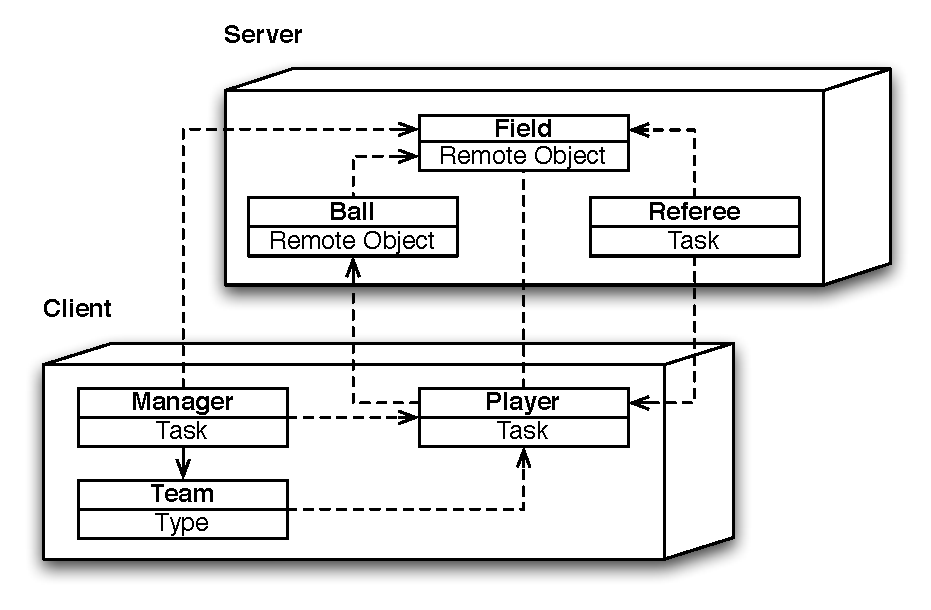
\includegraphics[width=250px]{images/distributed-system.pdf}
	\end{center}
\caption{Diagramma del sistema distribuito.}
\end{figure}

Per quanto riguarda la realizzazione del progetto, è stato sviluppato un modello Specifico per realizzare la distribuzione del sistema. Andiamo a vedere nel dettaglio di che cosa si tratta.

\subsection{Progettazione del Software Distribuito}

Il software distribuito \`e composto da tre entit\`a: una entit\`a servente che si occupa di generare una serie di eventi relativi all'avanzamento dello stato di gioco, una entit\`a che si occupa di gestire una coda nella quale vengono accodati gli eventi attraverso una funzione Push specifica e infine una entit\`a cliente che si occupa di visualizzare a terminale gli eventi accodati. \vspace{3mm}

La comunicazione tra le parti avviene attraverso la trasmissione di eventi legati all'avanzamento dello stato di gioco. 

\subsection{Struttura Distribuita delle Parti}

La struttura distribuita, come gi\`a menzionato \`e composta in linea generale da tre elementi funzionali:

\begin{itemize}
	\item \textbf{Server:} si occupa della generazione degli eventi sul campo di gioco;
	\item \textbf{Queue:} gestisce l'accodamento degli eventi ricevuti all'interno di una coda e rende disponibili due metodi Push e Pop che permettono di accedere attraverso inserimento ed estrazione;
	\item \textbf{Client:} permette la visualizzazione degli eventi generati dal server su molteplici display distribuiti;
\end{itemize}

Ognuno di essi \`e a sua volta composto da una serie di task necessari al corretto funzionamento della struttura. Andiamo ad analizzare nel dettaglio la composizione delle parti:

\begin{itemize}
	\item \textbf{Server:} genera e accoda eventi relativi allo stato di gioco:
		\begin{itemize}
			\item \textbf{Event Generator:} produce eventi casuali simulando la struttura di una partita reale;
			\item \textbf{Event Manager:} si occupa di "impacchettare" le informazioni ricevute dall'Event Generator per produrre un oggetto che sia trasmissibile al gestore della coda in modalit\`a remota. Per ognuno degli eventi ricevuti che corrispondono a particolari tipologie definite, si occupa anche della produzione di statistiche di gioco attraverso la chiamata di una procedura che modifica un record apposito;
		\end{itemize}
	\item \textbf{Queue:} attraverso 2 procedure protette \`e possibile effettuare l'inserimento (Push) in coda degli eventi prodotti e l'estrazione (Pop) degli stessi per accedere alle informazioni contenute nei pacchetti.
	\item \textbf{Client:} permette la visualizzazione degli eventi generati dal server su molteplici display distribuiti;
		\begin{itemize}
		\item \textbf{Event Display:} accede alla coda ed effettua l'estrazione degli eventi (se disponibili) e richiama la procedura per la stampa dell'evento a video;
		\item \textbf{Printer:} riceve i valori contenuti nell'evento e li manda a video attraverso i metodi canonici di stampa;
		\end{itemize}
\end{itemize}

\subsection{Trasmissione degli Eventi}

La trasmissione degli eventi avviene attraverso l'uso di oggetti di tipo Remote_Type e il passaggio degli stessi ad oggetti distribuiti sfruttando chiamate remote su package di tipo Remote_Procedure_Call. In questo modo \`e possibile mettere in comunicazione oggetti residenti su partizioni differenti in maniera del tutto trasparente rispetto al sistema. \vspace{3mm}

Andiamo ad analizzare nel dettaglio come avviene la comunicazione rispetto agli attori visti nella sezione precedente:





\subsection{}

\newpage

\section{Integrazione tra le Parti - Concorrenza e Distribuzione}

\begin{comment}
	
----------------------------------------------------------
----------------------------------------------------------
	
	
Presentiamo qui sopra lo schema con cui \`e composto il nostro sistema 

Le entit\`a principali sono fondamentalmente 6 di cui 3 risiedono sulla macchina server:

\begin{itemize}
	\item \textbf{Campo:} shared protected object;
	\item \textbf{Arbitro:} task;
	\item \textbf{Pallone:} shared protected object;
\end{itemize}

Le rimanenti sono proprie della squadra in gioco e risiedono sul client:

\begin{itemize}
	\item \textbf{Manager:} task;
	\item \textbf{Squadra:} shared protected object;
	\item \textbf{Giocatore:} task;
\end{itemize}

La comunicazione tra entit\'a avviene come indicato dai segmenti  che uniscono gli elementi presentati nella figura precedente. Viene inoltre indicato il verso in cui la comunicazione viene inizializzata, ovvero quale elemento si occupa di effettuare la chiamata di funzione/procedura che permette di interrogare lo stato degli elementi o modificare alcuni di essi. \vspace{3mm}

\subsection{Estensione del Modello Distribuito}

Potenzialmente risulta estremamente facile estendere il modello a partita singola in un campionato composto da una serie di squadre e una serie di singola partite. Il principio \`e quello di inserire un'ulteriore strato che si occupa di gestire il calendario, stabilendo gli incontri e gestendo i risultati al termine dei match al fine di gestire la classifica per decretare la formazione vincitrice. Il modello viene presentato nello schema sottostante:

\begin{figure}[H]
	\begin{center}
		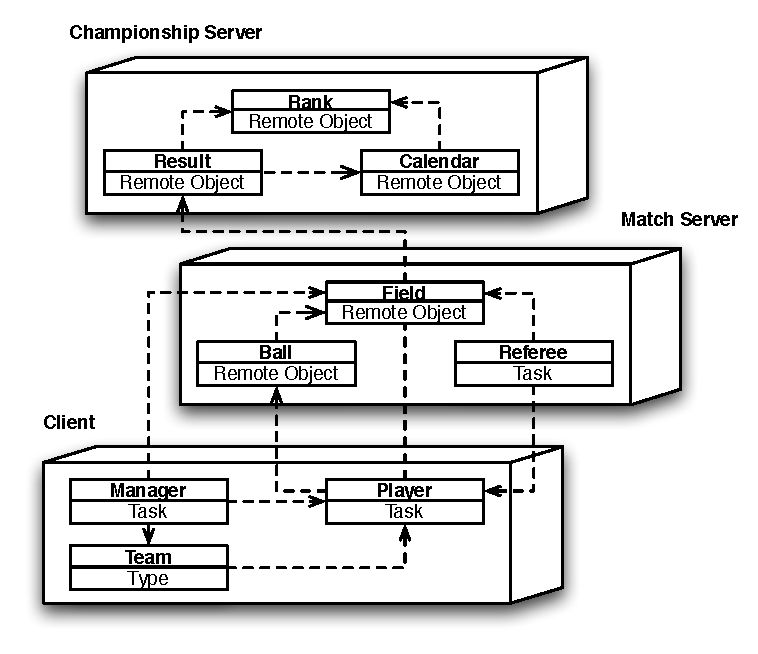
\includegraphics[width=260px]{images/distributed-championship.pdf}
	\end{center}
\caption{Diagramma del campionato distribuito.}
\end{figure}

\subsection{Creazione del Software Distribuito}

Attraverso l'utilizzo di Ada 95 DSA\footnote{Distributed System Annex}, la costruzione di un sistema distribuito \`e notevolmente semplificata per effetto dell'integrazione nello stesso linguaggio di programmazione di strutture di definizione di interfaccie che permettono di creare un sistema completamente distribuito senza dover ricorrere a linguaggli esterni (come ad esempio CORBA). \vspace{3mm}

I passaggi che permettono di realizzare in Ada 95 un sistema distribuito sono:

\begin{enumerate}
	\item Progettare un'applicazione come se non fosse distribuita;
	\item Identificare procedure remote (\emph{RPC}), variabili condivise (\emph{SP}) e oggeti distribuiti (\emph{RT}) e categorizzare i pacchetti;
	\item Realizzare e testare il sistema non distribuito;
	\item Redigere un file di configurazione (\emph{Configuration File}) per partizionare l'applicazione;
	\item Costruire le partizioni e testare l'applicazione distribuita.
\end{enumerate}

Avendo gi\`a sviluppato tutta l'applicazione come non distribuita, realizzarne la distribuzione si riduce all'identificazione delle entit\`a e alla ripartizione attraverso una configurazione. Nella box sottostante possiamo vedere il codice relativo al file di specificazione \verb=Configuration.ads=:  \vspace{3mm}

\lstset{language=Verilog, tabsize=3, backgroundcolor=\color{mygrey}, basicstyle=\small, commentstyle=\color{BrickRed}}
\lstinputlisting{code/Configuration.ads} \vspace{3mm}

In questo modo, come gi\`a visto, vengono creati gli stub di comunicazione tra client e server, il codice viene ripartito correttamente tr\`a le entit\`a e vengono generati gli eseguibili da utilizzare per il nostro gioco.

\subsection{Sincronizzazione Temporale}

Per poter gestire la partita su di un sistema completamente distribuito \`e fondamentale gestire la componente temporale. Ogni istanza, creata su macchine differenti, deve essere in grado di gestire in maniera autonoma il trascorrere del tempo. \vspace{3mm}

Anche in questo caso il linguaggio di programmazione ci viene incontro in quanto Ada 95 ci permette di accedere all'orologio di sistema e sfruttare sospensioni assolute per determinati intervalli temporali attraverso l'uso del package \verb=Ada.Real_Time=. Questa classe \`e in grado di fornire il controllo del tempo sulla base degli intervalli tra istanti temporali piuttosto che sul tempo orario. Come possiamo vedere nella figura sottostante, usare il tempo in maniera assoluta permette di gestire le sospensioni dei giocatori e garantire una durata unica di gioco per tutte le istanza clienti che partecipano alla partita. Ci viene inoltre in aiuto la classe ``Timer'' che si occupa di inizializzare contemporaneamente tutte le istanze dei processi attivi in gioco (giocatori e manager) e permette di decretare con lo stesso metodo il termine della partita.

\begin{figure}[H]
	\begin{center}
		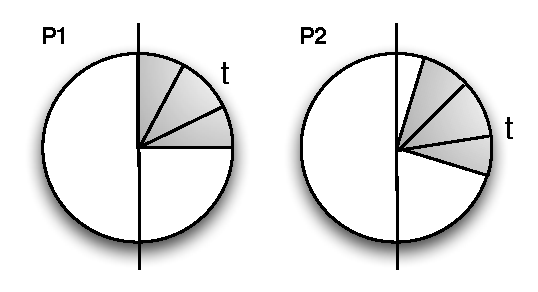
\includegraphics[width=250px]{images/time.pdf}
	\end{center}
\caption{Schema di avanzamento temporale nel gioco su macchine differenti.}
\end{figure}

Consideriamo una partita tipo: tutti i task vengono inizializzati e cominciano a lavorare contemporaneamente. A mano a mano che i singoli processi eseguono, vengono sospesi per \emph{n} istanti temporali, dove \emph{n} \`e un valore univoco e definito per tutti i calcolatori su cui viene distribuito il nostro sistema, assumendo come ipotesi che l'unit\`a temporale atomica \emph{t} intesa come istante sia definita univocamente per tutti i calcolatori. Il fatto che ogni orologio fisico non sia sincronizzato con quello degli altri calcolatori coinvolti non \`e un elemento fondamentale in quanto la correttezza del sistema \`e legata alla progressione degli istanti temporali \emph{t} relativi e non da orari definiti in senso assoluto. Ogni processo, dopo aver atteso il proprio turno nella coda dei processi pronti, prende il controllo della CPU, esegue il proprio lavoro e si autosospende usando la direttiva \verb=delay until= per $x \cdot n$ istanti temporali, dove \emph{x} dipende dalla velocit\`a di gioco del giocatore ed \emph{n} \`e appena stato definito. \vspace{3mm}

In Ada 95 il comando \verb=delay until= limita inferiormente la sospensione del processo garantendo attesa passiva fino allo scadere del tempo. Una volta risvegliato, il processo ritorna nella coda dei processi pronti, in attesa di eseguire nuovamente. Tali operazioni avvengono in maniera ciclica, fino allo scadere dei 90 minuti di gioco i quali riproporzionati su un equo valore di istanti temporali calcolati sulla base del rapporto tra tempo effettivo e tempo accelerato di gioco, nonch\`e in rapporto alla media delle sospensioni dei thread giocatori.

\subsection{Stati di Gioco}
\label{statidigioco}

Con stato di gioco si intende una procedura attraverso cui il server deve o meno ricordare lo stato del client al fine di poterlo riconoscere e procedere con eventuali azioni nei suoi confronti. Viene definito ``stateless'' un server che non ha necessit\`a di riconoscere la sessione con il client. Nel caso opposto il server viene definito come ``stateful''. \vspace{3mm}

Nel nostro caso possiamo definire il server come ``stateless''. Non c'\`e alcun motivo per cui debba memorizzare il client con il quale \`e connesso e neppure l'eventuale sessione. \vspace{3mm}

Tutti i client, indistintamente, si connettono con il server e in modo ciclico richiedono lo stato del campo e della palla. Una volta restituiti i dati i processi, in forma del tutto autonoma, processano le informazioni al fine di procedere con l'azione pi\`u corretta legata alle informazioni che hanno a disposizione e alle caratteristiche di ogni singolo giocatore. \vspace{3mm}

Una volta determinata la migliore azione, si connettono con il server, aprono una nuova sessione con la classe \emph{Field} per compiere il proprio movimento, eventualmente aprono una sessione con \emph{Ball} per effettuare modifiche allo stato del pallone e chiudono il collegamento. La trasmissione del proprio ID alla classe \emph{Field} permette di chiudere la sessione ed aprirne una nuova, minimizzando i tempi di collegamento. Nel caso in cui non venisse trasmesso l'ID del processo che deve effettuare la modifica, sarebbe necessario mantenere il collegamento dal momento della richiesta dello stato del campo fino alla trasmissione dell'aggiornamento. \vspace{3mm}

Questo per\`o porterebbe a tempi di trattenimento della risorsa potenzialmente elevati e quindi ad un blocco delle risorse in gioco e ad un conseguente ritardo nel ritmo della partita. \vspace{3mm}

\subsection{Sincronizzazione degli Stati}

A seguito di quanto appena visto nella sezione \ref{statodigioco} possiamo fare una integrazione andando ad analizzare gli effetti della trasmissione totale dello stato di gioco rispetto ad una trasmissione pi\`u compressa. \vspace{3mm}

Quando un processo si connette a \emph{Field} o a \emph{Ball} per effettuare richieste d'aggiornamento riceve in risposta un vettore contenente tutte le posizioni dei giocatori in campo e un vettore con la posizione del pallone. Una soluzione di questo genere pu\`o risultare alquanto dispendiosa, in quanto tra due richieste di aggiornamento effettuate dallo stesso processo ci possono essere giocatori che non hanno effettuato alcun movimento. In questo caso basterebbe comunicare la posizione dei giocatori che si sono mossi tra l'una e l'atra richiesta.

\begin{figure}[H]
	\begin{center}
		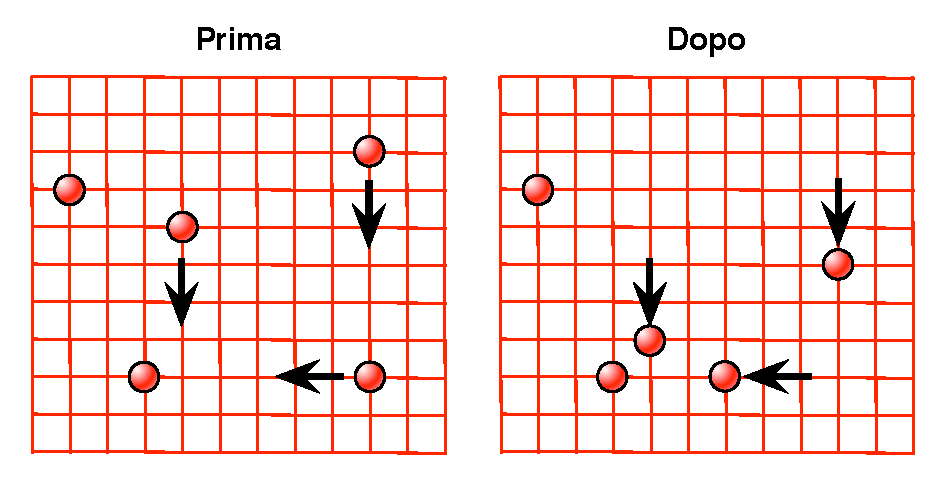
\includegraphics[width=350px]{images/state-transm.pdf}
	\end{center}
\caption{Schema di avanzamento di gioco con giocatori fermi.}
\end{figure}

Per implementare un'operazione di questo genere, basterebbe che \emph{Field} tenesse uno storico delle richieste e delle modifiche effettuate per poter comunicare tutti i movimenti che sono avvenuti nell'intervallo in questione. \vspace{3mm}

Ma se comunicare i $\Delta x$ movimenti tra una richiesta e l'altra pu\`o ottimizzare la banda con cui il nostro sistema distribuito comunica, \`e un metodo estremamente facile per portare il sistema ad uno stato di inconsistenza logica a seguito di un qualsiasi errore di trasmissione. Sarebbe inoltre necessario prevedere un meccanismo per tenere traccia di tutte le richieste effettuate da parte dei giocatori e implementare una lista, un array o un database in cui andare a registrare i vari spostamenti dei giocatori nel campo. Ai fini del nostro gioco, andrebbe senza ombra di dubbio ad appesantire una struttura progettuale che punta sulla semplicit\`a e sulla velocit\`a di gioco. \vspace{3mm}

Trasmettere l'instero stato del sistema ad ogni richiesta di variazioni, d'altro canto, permette di mantenere il sistema sempre sincronizzato attraverso il riposizionamento dei giocatori che hanno effettuato degli spostamenti e mantenendo in posizione coloro i quali abbiamo confermao non avere effettuato alcun movimento. Per effetto del fatto che \emph{Field} risulta una essere una risorsa protetta e quindi permette di modificare lo stato solo quando non ci sono operazioni di lettura in corso, il ``taglio'' del sistema che viene comunicato ai giocatori risulta essere consistente in quanto non ci sono operazioni di movimento che vengono ``tagliate'' in corso d'esecuzione.



----------------------------------------------------------
----------------------------------------------------------


\end{comment}




\newpage

\section{Codifica}

\subsection{Field}

\lstset{language=Verilog, tabsize=3, backgroundcolor=\color{mygrey}, basicstyle=\small, commentstyle=\color{BrickRed}}
\lstinputlisting{code/Field_Package.ads} 

\newpage

\subsection{Referee}

\lstset{language=Verilog, tabsize=3, backgroundcolor=\color{mygrey}, basicstyle=\small, commentstyle=\color{BrickRed}}
\lstinputlisting{code/Referee_Package.ads} 

\newpage

\subsection{Manager}

\lstset{language=Verilog, tabsize=3, backgroundcolor=\color{mygrey}, basicstyle=\small, commentstyle=\color{BrickRed}}
\lstinputlisting{code/Manager_Package.ads}

\newpage

\subsection{Player}

\lstset{language=Verilog, tabsize=3, backgroundcolor=\color{mygrey}, basicstyle=\small, commentstyle=\color{BrickRed}}
\lstinputlisting{code/Player_Package.ads}

\newpage

\subsection{Ball}

\lstset{language=Verilog, tabsize=3, backgroundcolor=\color{mygrey}, basicstyle=\small, commentstyle=\color{BrickRed}}
\lstinputlisting{code/Ball_Package.ads}

\newpage

\section{Conclusioni}

Il gioco proposto e dettagliato nei capitoli visti fino ad ora risponde a tutti i requisi presentati nella fase introduttiva e fornisce un buon supporto a concorrenza e distribuzione per effetto delle scelte progettuali messe in atto. \vspace{3mm}

Il modello di gioco \`e ridotto alle entit\`a base necessarie per il funzionamento del progetto. Tutti i processi sono formalmente corretti e adempiono ai loro compiti in modo semplice ed efficace. Le logiche di movimento e di gestione delle risorse che i giocatori applicano durante la partita sono anch'esse molto semplici ed estremamente funzionali. I manager dirigono il match favorendo strategie il pi\`u adatte alle situazioni in cui si pu\`o trovare lo scontro. L'arbitro, dal canto suo, viene richiamato da situazioni particolari e regola la partita attraverso scelte pi\`u o meno corrette, come in una partita reale. \vspace{3mm}

Come per ogni progetto, sono possibili migliorie alla strutture e agli algoritmi applicati al fine di perfezionare gli aspetti pi\`u grossolani e meno curati o eventuali errori non rilevati, ma ad una prima analisi il sistema \`e ben progettato. Nonostante la sua semplicit\`a, assolve a tutte le richieste. \`E alquanto probabile che un sistema pi\`u complesso e con scelte progettuali pi\`u estreme comporti un maggior rischio nel portare a situazioni non facilmente gestibili. In particolar modo si pu\`o incorrere in circostanze di forte concorrenza che portano inevitabilmente a situazioni di \emph{race condition}. La semplicit\`a del prodotto presentato permette di analizzare e risolvere facilmente tali situazioni attraverso soluzioni accademiche eleganti e logicamente corrette. \vspace{3mm}

La concorrenza tra giocatori \`e risolta attraverso la scelta del linguaggio di programmazione, Ada 95, e all'implementazione di risorse protette che ne garantiscono mutua esclusione. Vengono risolte le pi\`u comuni situazioni che portano il sistema ad uno stato di blocco parziale o totale, permettendo la costanza nel flusso di gioco. Anche la comunicazione tra processi avviene in sicurezza, utilizzando costrutti propri del linguaggio scelto. \vspace{3mm}

Non soltanto la concorrenza \`e stata oggetto di indagine. Anche la distribuzione del sistema ha comportato un lavoro dettagliato di analisi e ricerca delle soluzioni pi\`u adatte per permettere al sistema di funzionare anche se ridistribuito. La distribuzione, come la concorrenza, se non gestita in maniera appropriata rischia di portare a situazioni inconsistenti di gioco e alla corruzione della partita. Sono state prese in considerazione tutte le condizioni pi\`u comuni e sono state proposte e motivate soluzioni per risolvere i quesiti oggetto di discussione. \vspace{3mm}

Per quanto riguarda la codifica del prodotto, sono state tagliate le parti meno significative della specifica al fine di produrre in tempi contenuti un prototipo funzionante del sistema. Il modello cos\`i realizzato prevede lo svolgimento regolare della partita a cui vengono applicate regole di gioco semplificate, ma che riproducono effettivamente una simulazione funzionante. La codifica di tutte le regole trattate avrebbe comportato un aggravio dei tempi di produzione e di debug troppo oneroso per il gruppo (che allo stato attuale delle cose \`e composto da un solo elemento). Sono stati mantenuti comunque gli aspetti principali dei processi, definiti ed esaminati nella relazione.

\newpage

\section{Bibliografia}

\begin{thebibliography}{99}

\bibitem{ada95}
\emph{Ada Reference Manual},
2011.

\bibitem{burns07}
A. Burns, A. Wellings,
\emph{Concurrent and Real-time Programming in Ada},
Cambridge University Press,
3rd Edition,
2007.

\bibitem{tannenbaum06}
A. S. Tanenbaum, M. van Steen,
\emph{Distributed Systems: Principles and Paradigms},
Prentice Hall,
2nd Edition,
2006.

\bibitem{adaic}
Ada Resource Association
http://www.adaic.org/

\bibitem{adapower}
AdaPower.com - The Home of Ada,
http://www.adapower.com/

\bibitem{wikibooks}
Ada Programming, 
\emph{Wikibooks, open books for an open world}, 
http://en.wikibooks.org/

\end{thebibliography}

\end{document} % DONE WITH DOCUMENT!